% Options for packages loaded elsewhere
\PassOptionsToPackage{unicode}{hyperref}
\PassOptionsToPackage{hyphens}{url}
\PassOptionsToPackage{dvipsnames,svgnames,x11names}{xcolor}
%
\documentclass[
  11pt,
]{krantz}
\usepackage{amsmath,amssymb}
\usepackage{lmodern}
\usepackage{iftex}
\ifPDFTeX
  \usepackage[T1]{fontenc}
  \usepackage[utf8]{inputenc}
  \usepackage{textcomp} % provide euro and other symbols
\else % if luatex or xetex
  \usepackage{unicode-math}
  \defaultfontfeatures{Scale=MatchLowercase}
  \defaultfontfeatures[\rmfamily]{Ligatures=TeX,Scale=1}
  \setmonofont[Scale=0.775]{MesloLGS NF}
\fi
% Use upquote if available, for straight quotes in verbatim environments
\IfFileExists{upquote.sty}{\usepackage{upquote}}{}
\IfFileExists{microtype.sty}{% use microtype if available
  \usepackage[]{microtype}
  \UseMicrotypeSet[protrusion]{basicmath} % disable protrusion for tt fonts
}{}
\makeatletter
\@ifundefined{KOMAClassName}{% if non-KOMA class
  \IfFileExists{parskip.sty}{%
    \usepackage{parskip}
  }{% else
    \setlength{\parindent}{0pt}
    \setlength{\parskip}{6pt plus 2pt minus 1pt}}
}{% if KOMA class
  \KOMAoptions{parskip=half}}
\makeatother
\usepackage{xcolor}
\IfFileExists{xurl.sty}{\usepackage{xurl}}{} % add URL line breaks if available
\IfFileExists{bookmark.sty}{\usepackage{bookmark}}{\usepackage{hyperref}}
\hypersetup{
  pdftitle={Data Science per psicologi},
  pdfauthor={Corrado Caudek},
  colorlinks=true,
  linkcolor={Maroon},
  filecolor={Maroon},
  citecolor={Blue},
  urlcolor={Blue},
  pdfcreator={LaTeX via pandoc}}
\urlstyle{same} % disable monospaced font for URLs
\usepackage{color}
\usepackage{fancyvrb}
\newcommand{\VerbBar}{|}
\newcommand{\VERB}{\Verb[commandchars=\\\{\}]}
\DefineVerbatimEnvironment{Highlighting}{Verbatim}{commandchars=\\\{\}}
% Add ',fontsize=\small' for more characters per line
\usepackage{framed}
\definecolor{shadecolor}{RGB}{248,248,248}
\newenvironment{Shaded}{\begin{snugshade}}{\end{snugshade}}
\newcommand{\AlertTok}[1]{\textcolor[rgb]{0.33,0.33,0.33}{#1}}
\newcommand{\AnnotationTok}[1]{\textcolor[rgb]{0.37,0.37,0.37}{\textbf{\textit{#1}}}}
\newcommand{\AttributeTok}[1]{\textcolor[rgb]{0.61,0.61,0.61}{#1}}
\newcommand{\BaseNTok}[1]{\textcolor[rgb]{0.06,0.06,0.06}{#1}}
\newcommand{\BuiltInTok}[1]{#1}
\newcommand{\CharTok}[1]{\textcolor[rgb]{0.5,0.5,0.5}{#1}}
\newcommand{\CommentTok}[1]{\textcolor[rgb]{0.37,0.37,0.37}{\textit{#1}}}
\newcommand{\CommentVarTok}[1]{\textcolor[rgb]{0.37,0.37,0.37}{\textbf{\textit{#1}}}}
\newcommand{\ConstantTok}[1]{\textcolor[rgb]{0,0,0}{#1}}
\newcommand{\ControlFlowTok}[1]{\textcolor[rgb]{0.27,0.27,0.27}{\textbf{#1}}}
\newcommand{\DataTypeTok}[1]{\textcolor[rgb]{0.27,0.27,0.27}{#1}}
\newcommand{\DecValTok}[1]{\textcolor[rgb]{0.06,0.06,0.06}{#1}}
\newcommand{\DocumentationTok}[1]{\textcolor[rgb]{0.37,0.37,0.37}{\textbf{\textit{#1}}}}
\newcommand{\ErrorTok}[1]{\textcolor[rgb]{0.14,0.14,0.14}{\textbf{#1}}}
\newcommand{\ExtensionTok}[1]{#1}
\newcommand{\FloatTok}[1]{\textcolor[rgb]{0.06,0.06,0.06}{#1}}
\newcommand{\FunctionTok}[1]{\textcolor[rgb]{0,0,0}{#1}}
\newcommand{\ImportTok}[1]{#1}
\newcommand{\InformationTok}[1]{\textcolor[rgb]{0.37,0.37,0.37}{\textbf{\textit{#1}}}}
\newcommand{\KeywordTok}[1]{\textcolor[rgb]{0.27,0.27,0.27}{\textbf{#1}}}
\newcommand{\NormalTok}[1]{#1}
\newcommand{\OperatorTok}[1]{\textcolor[rgb]{0.43,0.43,0.43}{\textbf{#1}}}
\newcommand{\OtherTok}[1]{\textcolor[rgb]{0.37,0.37,0.37}{#1}}
\newcommand{\PreprocessorTok}[1]{\textcolor[rgb]{0.37,0.37,0.37}{\textit{#1}}}
\newcommand{\RegionMarkerTok}[1]{#1}
\newcommand{\SpecialCharTok}[1]{\textcolor[rgb]{0,0,0}{#1}}
\newcommand{\SpecialStringTok}[1]{\textcolor[rgb]{0.5,0.5,0.5}{#1}}
\newcommand{\StringTok}[1]{\textcolor[rgb]{0.5,0.5,0.5}{#1}}
\newcommand{\VariableTok}[1]{\textcolor[rgb]{0,0,0}{#1}}
\newcommand{\VerbatimStringTok}[1]{\textcolor[rgb]{0.5,0.5,0.5}{#1}}
\newcommand{\WarningTok}[1]{\textcolor[rgb]{0.37,0.37,0.37}{\textbf{\textit{#1}}}}
\usepackage{longtable,booktabs,array}
\usepackage{calc} % for calculating minipage widths
% Correct order of tables after \paragraph or \subparagraph
\usepackage{etoolbox}
\makeatletter
\patchcmd\longtable{\par}{\if@noskipsec\mbox{}\fi\par}{}{}
\makeatother
% Allow footnotes in longtable head/foot
\IfFileExists{footnotehyper.sty}{\usepackage{footnotehyper}}{\usepackage{footnote}}
\makesavenoteenv{longtable}
\usepackage{graphicx}
\makeatletter
\def\maxwidth{\ifdim\Gin@nat@width>\linewidth\linewidth\else\Gin@nat@width\fi}
\def\maxheight{\ifdim\Gin@nat@height>\textheight\textheight\else\Gin@nat@height\fi}
\makeatother
% Scale images if necessary, so that they will not overflow the page
% margins by default, and it is still possible to overwrite the defaults
% using explicit options in \includegraphics[width, height, ...]{}
\setkeys{Gin}{width=\maxwidth,height=\maxheight,keepaspectratio}
% Set default figure placement to htbp
\makeatletter
\def\fps@figure{htbp}
\makeatother
\setlength{\emergencystretch}{3em} % prevent overfull lines
\providecommand{\tightlist}{%
  \setlength{\itemsep}{0pt}\setlength{\parskip}{0pt}}
\setcounter{secnumdepth}{5}
\usepackage{amsmath}
\usepackage{amssymb}
\usepackage{amsfonts}

\defaultfontfeatures{Scale=MatchLowercase}

\usepackage{booktabs}
\usepackage{longtable}
\usepackage[bf,singlelinecheck=off]{caption}

\usepackage{framed,color}
\definecolor{shadecolor}{RGB}{248,248,248}

\renewcommand{\textfraction}{0.05}
\renewcommand{\topfraction}{0.8}
\renewcommand{\bottomfraction}{0.8}
\renewcommand{\floatpagefraction}{0.75}

\renewenvironment{quote}{\begin{VF}}{\end{VF}}
\let\oldhref\href
\renewcommand{\href}[2]{#2\footnote{\url{#1}}}

\ifxetex
  \usepackage{letltxmacro}
  \setlength{\XeTeXLinkMargin}{1pt}
  \LetLtxMacro\SavedIncludeGraphics\includegraphics
  \def\includegraphics#1#{% #1 catches optional stuff (star/opt. arg.)
    \IncludeGraphicsAux{#1}%
  }%
  \newcommand*{\IncludeGraphicsAux}[2]{%
    \XeTeXLinkBox{%
      \SavedIncludeGraphics#1{#2}%
    }%
  }%
\fi

\makeatletter
\newenvironment{kframe}{%
\medskip{}
\setlength{\fboxsep}{.8em}
 \def\at@end@of@kframe{}%
 \ifinner\ifhmode%
  \def\at@end@of@kframe{\end{minipage}}%
  \begin{minipage}{\columnwidth}%
 \fi\fi%
 \def\FrameCommand##1{\hskip\@totalleftmargin \hskip-\fboxsep
 \colorbox{shadecolor}{##1}\hskip-\fboxsep
     % There is no \\@totalrightmargin, so:
     \hskip-\linewidth \hskip-\@totalleftmargin \hskip\columnwidth}%
 \MakeFramed {\advance\hsize-\width
   \@totalleftmargin\z@ \linewidth\hsize
   \@setminipage}}%
 {\par\unskip\endMakeFramed%
 \at@end@of@kframe}
\makeatother

\renewenvironment{Shaded}{\begin{kframe}}{\end{kframe}}

\usepackage{makeidx}
\makeindex

\urlstyle{tt}

\usepackage{amsthm}
\makeatletter
\def\thm@space@setup{%
  \thm@preskip=8pt plus 2pt minus 4pt
  \thm@postskip=\thm@preskip
}
\makeatother

\DeclareMathOperator{\Var}{\mathbb{V}} % Define variance operator
\DeclareMathOperator{\SD}{SD} % Define sd operator
\DeclareMathOperator{\Cov}{Cov} % Define covariance operator
\DeclareMathOperator{\Corr}{Corr} % Define correlation operator
\DeclareMathOperator{\Me}{Me} % Define mediane operator
\DeclareMathOperator{\Mo}{Mo} % Define mode operator

\DeclareMathOperator{\Bin}{Binomial} % Define binomial operator
\DeclareMathOperator{\Bernoulli}{Bernoulli} % Define Bernoulli operator
\DeclareMathOperator{\Ber}{\mathscr{B}} % Define Bernoulli operator
\DeclareMathOperator{\Poi}{Poisson} % Define Poisson operator
\DeclareMathOperator{\Uniform}{Uniform} % Define Uniform operator
\DeclareMathOperator{\Cauchy}{Cauchy} % Define Cauchy operator
\DeclareMathOperator{\B}{B} % beta function
% \mbox{B}(a, b) % beta function
% \mbox{Beta}(a, b) % beta distribution

\DeclareMathOperator{\elpd}{elpd} % Define elpd operator
\DeclareMathOperator{\lppd}{lppd} % Define lppd operator
\DeclareMathOperator{\LOO}{LOO} % Define LOO operator
\DeclareMathOperator{\argmin}{arg\,min} 
\DeclareMathOperator{\argmax}{arg\,max} 

\newcommand{\E}{\mathbb{E}} % Define expected value operator
\newcommand{\R}{\textsf{R}} % Define R programming language symbol
\newcommand{\Real}{\mathbb{R}} % Define real number operator
\newcommand{\Prob}{\mathscr{P}}
\newcommand{\indep}{\perp \!\!\! \perp}

\usepackage[
 labelfont=bf,
 font={small, it}
]{caption}
\usepackage{upquote} % print correct quotes in verbatim-environments
\usepackage{empheq}
\usepackage{xfrac}

\usepackage{polyglossia}
\setmainlanguage{italian}

\frontmatter
\ifLuaTeX
  \usepackage{selnolig}  % disable illegal ligatures
\fi
\usepackage[]{natbib}
\bibliographystyle{apalike}

\title{Data Science per psicologi}
\author{Corrado Caudek}
\date{2022-02-08}

\usepackage{amsthm}
\newtheorem{theorem}{Teorema}[chapter]
\newtheorem{lemma}{Lemma}[chapter]
\newtheorem{corollary}{Corollario}[chapter]
\newtheorem{proposition}{Proposizione}[chapter]
\newtheorem{conjecture}{Congettura}[chapter]
\theoremstyle{definition}
\newtheorem{definition}{Definizione}[chapter]
\theoremstyle{definition}
\newtheorem{example}{Esempio}[chapter]
\theoremstyle{definition}
\newtheorem{exercise}{Esercizio}[chapter]
\theoremstyle{definition}
\newtheorem{hypothesis}{Hypothesis}[chapter]
\theoremstyle{remark}
\newtheorem*{remark}{Osservazione}
\newtheorem*{solution}{Soluzione}
\begin{document}
\maketitle

\cleardoublepage\newpage\thispagestyle{empty}\null
% \cleardoublepage\newpage\thispagestyle{empty}\null
%\cleardoublepage\newpage
\thispagestyle{empty}
\begin{center}
\Large{Psicometria -- AA 2021/2022}

\vskip20pt

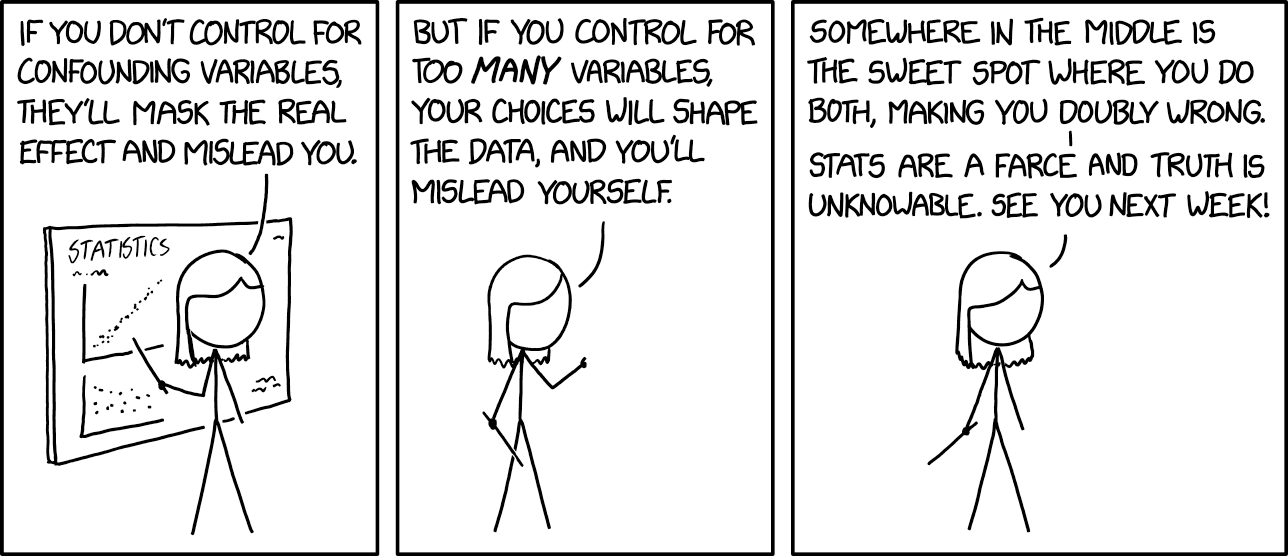
\includegraphics{images/confounding_variables.png}
\end{center}

\setlength{\abovedisplayskip}{-5pt}
\setlength{\abovedisplayshortskip}{-5pt}

{
\hypersetup{linkcolor=}
\setcounter{tocdepth}{2}
\tableofcontents
}
\listoffigures
\listoftables
\hypertarget{prefazione}{%
\chapter*{Prefazione}\label{prefazione}}


\emph{Data Science per psicologi} contiene il materiale delle lezioni dell'insegnamento di \emph{Psicometria B000286} (A.A. 2021/2022) rivolto agli studenti del primo anno del Corso di Laurea in Scienze e Tecniche Psicologiche dell'Università degli Studi di Firenze. \emph{Psicometria} si propone di fornire agli studenti un'introduzione all'analisi dei dati in psicologia. Le conoscenze/competenze che verranno sviluppate in questo insegnamento sono quelle della Data science, ovvero un insieme di conoscenze/competenze che si pongono all'intersezione tra statistica (ovvero, richiedono la capacità di comprendere teoremi statistici) e informatica (ovvero, richiedono la capacità di sapere utilizzare un software).

\hypertarget{la-psicologia-e-la-data-science}{%
\section*{La psicologia e la Data science}\label{la-psicologia-e-la-data-science}}


Sembra sensato spendere due parole su un tema che è importante per gli studenti: quello indicato dal titolo di questo Capitolo. È ovvio che agli studenti di psicologia la statistica non piace. Se piacesse, forse studierebbero Data science e non psicologia; ma non lo fanno. Di conseguenza, gli studenti di psicologia si chiedono: ``perché dobbiamo perdere tanto tempo a studiare queste cose quando in realtà quello che ci interessa è tutt'altro?'' Questa è una bella domanda.

C'è una ragione molto semplice che dovrebbe farci capire perché la Data science è così importante per la psicologia. Infatti, a ben pensarci, la psicologia è una disciplina intrinsecamente statistica, se per statistica intendiamo quella disciplina che studia la variazione delle caratteristiche degli individui nella popolazione. La psicologia studia \emph{gli individui} ed è proprio la variabilità inter- e intra-individuale ciò che vogliamo descrivere e, in certi casi, predire. In questo senso, la psicologia è molto diversa dall'ingegneria, per esempio. Le proprietà di un determinato ponte sotto certe condizioni, ad esempio, sono molto simili a quelle di un altro ponte, sotto le medesime condizioni. Quindi, per un ingegnere la statistica è poco importante: le proprietà dei materiali sono unicamente dipendenti dalla loro composizione e restano costanti. Ma lo stesso non può dirsi degli individui: ogni individuo è unico e cambia nel tempo. E le variazioni tra gli individui, e di un individuo nel tempo, sono l'oggetto di studio proprio della psicologia: è dunque chiaro che i problemi che la psicologia si pone sono molto diversi da quelli affrontati, per esempio, dagli ingegneri. Questa è la ragione per cui abbiamo tanto bisogno della Data science in psicologia: perché la Data science ci consente di descrivere la variazione e il cambiamento. E queste sono appunto le caratteristiche di base dei fenomeni psicologici.

Sono sicuro che, leggendo queste righe, a molti studenti sarà venuta in mente la seguente domanda: perché non chiediamo a qualche esperto di fare il ``lavoro sporco'' (ovvero le analisi statistiche) per noi, mentre noi (gli psicologi) ci occupiamo solo di ciò che ci interessa, ovvero dei problemi psicologici slegati dai dettagli ``tecnici'' della Data science? La risposta a questa domanda è che non è possibile progettare uno studio psicologico sensato senza avere almeno una comprensione rudimentale della Data science. Le tematiche della Data science non possono essere ignorate né dai ricercatori in psicologia né da coloro che svolgono la professione di psicologo al di fuori dell'Università. Infatti, anche i professionisti al di fuori dall'università non possono fare a meno di leggere la letteratura psicologica più recente: il continuo aggiornamento delle conoscenze è infatti richiesto dalla deontologia della professione. Ma per potere fare questo è necessario conoscere un bel po' di Data science! Basta aprire a caso una rivista specialistica di psicologia per rendersi conto di quanto ciò sia vero: gli articoli che riportano i risultati delle ricerche psicologiche sono zeppi di analisi statistiche e di modelli formali. E la comprensione della letteratura psicologica rappresenta un requisito minimo nel bagaglio professionale dello psicologo.

Le considerazioni precedenti cercano di chiarire il seguente punto: la Data science non è qualcosa da studiare a malincuore, in un singolo insegnamento universitario, per poi poterla tranquillamente dimenticare. Nel bene e nel male, gli psicologi usano gli strumenti della Data science in tantissimi ambiti della loro attività professionale: in particolare quando costruiscono, somministrano e interpretano i test psicometrici. È dunque chiaro che possedere delle solide basi di Data science è un tassello imprescindibile del bagaglio professionale dello psicologo. In questo insegnamento verrano trattati i temi base della Data science e verrà adottato un punto di vista bayesiano, che corrisponde all'approccio più recente e sempre più diffuso in psicologia.

\hypertarget{come-studiare}{%
\section*{Come studiare}\label{come-studiare}}


Il giusto metodo di studio per prepararsi all'esame di Psicometria è quello di seguire attivamente le lezioni, assimilare i concetti via via che essi vengono presentati e verificare in autonomia le procedure presentate a lezione. Incoraggio gli studenti a farmi domande per chiarire ciò che non è stato capito appieno. Incoraggio gli studenti a utilizzare i forum attivi su Moodle e, soprattutto, a svolgere gli esercizi proposti su Moodle. I problemi forniti su Moodle rappresentano il livello di difficoltà richiesto per superare l'esame e consentono allo studente di comprendere se le competenze sviluppate fino a quel punto sono sufficienti rispetto alle richieste dell'esame.

La prima fase dello studio, che è sicuramente individuale, è quella in cui è necessario acquisire le conoscenze teoriche relative ai problemi che saranno presentati all'esame. La seconda fase di studio, che può essere facilitata da scambi con altri e da incontri di gruppo, porta ad acquisire la capacità di applicare le conoscenze: è necessario capire come usare un software (\(\textsf{R}\)) per applicare i concetti statistici alla specifica situazione del problema che si vuole risolvere. Le due fasi non sono però separate: il saper fare molto spesso ci aiuta a capire meglio.

\hypertarget{sviluppare-un-metodo-di-studio-efficace}{%
\section*{Sviluppare un metodo di studio efficace}\label{sviluppare-un-metodo-di-studio-efficace}}


Avendo insegnato molte volte in passato un corso introduttivo di analisi dei dati ho notato nel corso degli anni che gli studenti con l'atteggiamento mentale che descriverò qui sotto generalmente ottengono ottimi risultati. Alcuni studenti sviluppano naturalmente questo approccio allo studio, ma altri hanno bisogno di fare uno sforzo per maturarlo. Fornisco qui sotto una breve descrizione del ``metodo di studio'' che, nella mia esperienza, è il più efficace per affrontare le richieste di questo insegnamento.

\begin{itemize}
\tightlist
\item
  Dedicate un tempo sufficiente al materiale di base, apparentemente facile; assicuratevi di averlo capito bene. Cercate le lacune nella vostra comprensione. Leggere presentazioni diverse dello stesso materiale (in libri o articoli diversi) può fornire nuove intuizioni.
\item
  Gli errori che facciamo sono i nostri migliori maestri. Istintivamente cerchiamo di dimenticare subito i nostri errori. Ma il miglior modo di imparare è apprendere dagli errori che commettiamo. In questo senso, una soluzione corretta è meno utile di una soluzione sbagliata. Quando commettiamo un errore questo ci fornisce un'informazione importante: ci fa capire qual è il materiale di studio sul quale dobbiamo ritornare e che dobbiamo capire meglio.
\item
  C'è ovviamente un aspetto ``psicologico'' nello studio. Quando un esercizio o problema ci sembra incomprensibile, la cosa migliore da fare è dire: ``mi arrendo'', ``non ho idea di cosa fare!''. Questo ci rilassa: ci siamo già arresi, quindi non abbiamo niente da perdere, non dobbiamo più preoccuparci. Ma non dobbiamo fermarci qui. Le cose ``migliori'' che faccio (se ci sono) le faccio quando non ho voglia di lavorare. Alle volte, quando c'è qualcosa che non so fare e non ho idea di come affontare, mi dico: ``oggi non ho proprio voglia di fare fatica'', non ho voglia di mettermi nello stato mentale per cui ``in 10 minuti devo risolvere il problema perché dopo devo fare altre cose''. Però ho voglia di \emph{divertirmi} con quel problema e allora mi dedico a qualche aspetto ``marginale'' del problema, che so come affrontare, oppure considero l'aspetto più difficile del problema, quello che non so come risolvere, ma invece di cercare di risolverlo, guardo come altre persone hanno affrontato problemi simili, opppure lo stesso problema in un altro contesto. Non mi pongo l'obiettivo ``risolvi il problema in 10 minuti'', ma invece quello di farmi un'idea ``generale'' del problema, o quello di capire un caso più specifico e più semplice del problema. Senza nessuna pressione. Infatti, in quel momento ho deciso di non lavorare (ovvero, di non fare fatica). Va benissimo se ``parto per la tangente'', ovvero se mi metto a leggere del materiale che sembra avere poco a che fare con il problema centrale (le nostre intuizioni e la nostra curiosità solitamente ci indirizzano sulla strada giusta). Quando faccio così, molto spesso trovo la soluzione del problema che mi ero posto e, paradossalmente, la trovo in un tempo minore di quello che, in precedenza, avevo dedicato a ``lavorare'' al problema. Allora perché non faccio sempre così? C'è ovviamente l'aspetto dei ``10 minuti'' che non è sempre facile da dimenticare. Sotto pressione, possiamo solo agire in maniera automatica, ovvero possiamo solo applicare qualcosa che già sappiamo fare. Ma se dobbiamo imparare qualcosa di nuovo, la pressione è un impedimento.
\item
  È utile farsi da soli delle domande sugli argomenti trattati, senza limitarsi a cercare di risolvere gli esercizi che vengono assegnati. Quando studio qualcosa mi viene in mente: ``se questo è vero, allora deve succedere quest'altra cosa''. Allora verifico se questo è vero, di solito con una simulazione. Se i risultati della simulazione sono quelli che mi aspetto, allora vuol dire che ho capito. Se i risultati sono diversi da quelli che mi aspettavo, allora mi rendo conto di non avere capito e ritorno indietro a studiare con più attenzione la teoria che pensavo di avere capito -- e ovviamente mi rendo conto che c'era un aspetto che avevo frainteso. Questo tipo di verifica è qualcosa che dobbiamo fare da soli, in prima persona: nessun altro può fare questo al posto nostro.
\item
  Non aspettatevi di capire tutto la prima volta che incontrate un argomento nuovo.\footnote{Ricordatevi inoltre che gli individui tendono a sottostimare la propria capacità di apprendere \citep{horn2021underestimating}.} È utile farsi una nota mentalmente delle lacune nella vostra comprensione e tornare su di esse in seguito per carcare di colmarle. L'atteggiamento naturale, quando non capiamo i dettagli di qualcosa, è quello di pensare: ``non importa, ho capito in maniera approssimativa questo punto, non devo preoccuparmi del resto''. Ma in realtà non è vero: se la nostra comprensione è superficiale, quando il problema verrà presentato in una nuova forma, non riusciremo a risolverlo. Per cui i dubbi che ci vengono quando studiamo qualcosa sono il nostro alleato più prezioso: ci dicono esattamente quali sono gli aspetti che dobbiamo approfondire per potere migliorare la nostra preparazione.
\item
  È utile sviluppare una visione d'insieme degli argomenti trattati, capire l'obiettivo generale che si vuole raggiungere e avere chiaro il contributo che i vari pezzi di informazione forniscono al raggiungimento di tale obiettivo. Questa organizzazione mentale del materiale di studio facilita la comprensione. È estremamente utile creare degli schemi di ciò che si sta studiando. Non aspettate che sia io a fornirvi un riepilogo di ciò che dovete imparare: sviluppate da soli tali schemi e tali riassunti.
\item
  Tutti noi dobbiamo imparare l'arte di trovare le informazioni, non solo nel caso di questo insegnamento. Quando vi trovate di fronte a qualcosa che non capite, o ottenete un oscuro messaggio di errore da un software, ricordatevi: ``Google is your friend''!
\end{itemize}

\begin{flushright}
Corrado Caudek\\
Marzo 2022 \end{flushright}

\mainmatter

\hypertarget{part-il-calcolo-delle-probabilituxe0}{%
\part{Il calcolo delle probabilità}\label{part-il-calcolo-delle-probabilituxe0}}

\hypertarget{intro-prob-1}{%
\chapter{Il ragionamento scientifico: deduzione e induzione}\label{intro-prob-1}}

In questa parte della dispensa verrà introdotta la teoria delle probabilità. Prima di entrare nei dettagli, cerchiamo di capire perché la probabilità sia cruciale per la ricerca scientifica. Ingenuamente, potremmo pensare che la logica deduttiva (aristotelica) fornisca il modo migliore di procedere alla ricerca scientifica -- con un tale metodo, infatti, non si commettono errori. Un esempio di tale logica è il sillogismo, come ad esempio,

\begin{itemize}
\tightlist
\item
  tutti gli uomini sono mortali,
\item
  Socrate è un uomo,
\item
  quindi, Socrate è mortale.
\end{itemize}

La logica deduttiva, però, non può essere utilizzata in psicologia, né in alcun'altra scienza empirica. Nel sillogismo, la correttezza del ragionamento dipende dalla sua struttura e non dal significato delle parole (come uomo, mortale, ecc.). Nelle scienze empiriche, però, il ``significato delle parole'' è cruciale. Le ``parole'' usate nel sillogismo corrispondono ai ``concetti teorici'' (detti, in psicologia, costrutti) delle teorie scientifiche. Il problema è che la \emph{corrispondenza} tra le relazioni tra costrutti teorici, da una parte, e le relazioni tra i fenomeni empirici, dall'altra, dipende dalla validità delle teorie. In fisica, ad esempio, i concetti teorici di massa (\(m\)), peso (\(P\)) e forza di gravità (\(g\)) consentono di descrivere accuratamente ciò che si osserva nel mondo empirico: \(P = m \cdot g\). Non è così, invece, nelle scienze sociali, dove le relazioni tra costrutti sono in grado di descrivere \emph{solo in parte} le relazioni tra i corrispondenti fenomeni empirici. Nelle scienze sociali, dunque, la ricerca procede mediante l'inferenza induttiva. Non siamo mai completamente sicuri della verità di una proposizione: al valore di verità di una proposizione possiamo solo assegnare un giudizio probabilistico. L'approccio bayesiano è una scuola di pensiero che usa la probabilità per quantificare il grado di credenza che viene attribuito al valore di verità di una proposizione. L'inferenza statistica bayesiana è dunque un tipo di inferenza induttiva, ovvero è un insieme di procedure che hanno lo scopo di quantificare quanto sia plausibile la proposizione \(A\) dopo aver osservato l'evento \(B\). Per svolgere l'inferenza statistica bayesiana è dunque necessario quantificare la plausibilità che viene attribuita ad una proposizione e lo strumento che consente di fare questo è la teoria delle probabilità. Una discussione dell'inferenza statistica bayesiana richiede dunque, preliminarmente, la conoscenze della teoria delle probabilità.

\hypertarget{proposizioni-e-modelli-statistici}{%
\section{Proposizioni e modelli statistici}\label{proposizioni-e-modelli-statistici}}

Vedremo che, nell'inferenza bayesiana, le proposizioni di una teoria scientifica sono espresse nella forma di un modello statistico, ovvero mediante una legge generale che descrive il modo in cui un fenomeno si manifesta. Tale legge generale viene anche detta \emph{processo generativo dei dati}, o modello statistico. Ma che cos'è un modello generativo dei dati? Per fare un esempio, consideriamo il quoziente d'intelligenza. Sappiamo che il punteggio totale della \emph{Wechsler Adult Intelligence Scale} ha, nella popolazione, media 100 e deviazione standard 15 (dato che il test WAIS è stato costruito in modo da avere una tale proprietà). Quindi, se prendiamo un campione abbastanza grande di persone, i valori del QI di tali persone avranno, circa, media uguale a 100 e deviazione standard uguale a 15. Se con tali dati costruiamo un istogramma, sappiamo anche che il profilo di tale istogramma sarà ben descritto da una funzione matematica che va sotto il nome di \emph{legge gaussiana}. La rappresentazione grafica della funzione gaussiana è la classica curva a campana che avrete visto tante volte in passato. La funzione gaussiana dipende da due parametri: la media (solitamente indicata con \(\mu\)) e la deviazione standard (\(\sigma\)). Se cambiamo questi parametri, ma usiamo sempre la stessa formula, otteniamo una curva diversa. Per esempio, se consideriamo solo la sotto-popolazione dei bambini plus-dotati, la distribuzione dei punteggi QI sarà una gaussiana centrata su 130, con una qualche deviazione standard. In questo esempio, la gaussiana è il modello generatore dei dati e i parametri sono \(\mu\) e \(\sigma\). Per altri fenomeni, come ad esempio i tempi di reazione nel compito Stroop, o la gravità della sintomatologia ansiosa negli adulti misurata attraverso il test \emph{Beck Anxiety Inventory}, il modello gaussiano non è più appropriato ed è necessario \emph{ipotizzare} un diverso processo generatore dei dati.

In generale, l'inferenza induttiva bayesiana procede \emph{ipotizzando} un modello generatore dei dati per poi, sulla base dei dati osservati in un campione e sulla base delle nostre credenze a priori, \emph{inferire} i valori plausibili dei parametri del modello. In questo processo inferenziale, possiamo individuare cinque fonti di incertezza:

\begin{enumerate}
\def\labelenumi{\arabic{enumi}.}
\tightlist
\item
  incertezza sui parametri dei modelli;
\item
  incertezza su quale sia il modello migliore;
\item
  incertezza su cosa fare con l'output dei (migliori) modelli;
\item
  incertezza sul funzionamento del software che produce i risultati;
\item
  incertezza sul fatto che il/i modello/i (migliore/i) siano coerenti con altri campioni di dati.
\end{enumerate}

\begin{itemize}
\tightlist
\item
  L'approccio bayesiano usa la teoria delle probabilità per descrivere l'incertezza relativa ai punti (1) e (2);
\item
  l'approccio bayesiano si collega alla teoria delle decisioni, che prescrive come affrontare il problema descritto nel punto (3);
\item
  il software utilizzato (nel nostro caso, Stan) fa tutto ciò che è possibile per mitigare la preoccupazione (4);
\item
  l'approccio bayesiano consente di quantificare l'incertezza descritta al punto (5).
\end{itemize}

\hypertarget{oggettivituxe0-e-soggettivituxe0}{%
\section{Oggettività e soggettività}\label{oggettivituxe0-e-soggettivituxe0}}

Facendo delle assunzioni non controverse, l'inferenza bayesiana consente di aggiornare le credenze precedenti sui valori (sconosciuti) dei parametri \(\theta\) di un modello statistico alla luce di nuovi dati \(y_1, y_2, \dots, y_N\) che vengono osservati. L'approccio bayesiano è etichettato come ``soggettivo'' perché non ci dice quale valore dovrebbe essere assegnato ai parametri prima di avere osservato i dati \(y_1, y_2, \dots, y_N\). In realtà, l'aggiornamento bayesiano è il modo più razionale di procedere: se, prima di avere osservato i dati, il ricercatore ha una credenza assurda relativamente al valore di \(\theta\), dopo avere osservato \(y_1, y_2, \dots, y_N\) le sue credenze su \(\theta\) aggiornate secondo i principi bayesiani saranno meno assurde. Il problema di questo modo di procedere non è che, a priori, i ricercatori (o chiunque) possono avere delle credenze sbagliate, ma bensì il fatto che, quando osservano \(y_1, y_2, \dots, y_N\), non aggiornano le loro credenze su \(\theta\) secondo i principi bayesiani. Infatti, in alcune situazioni, l'osservazione di dati che contraddicono le credenze precedenti non fa altro che rafforzare tali convinzioni errate -- il problema, dunque, non nasce dalla ``soggettività'' dell'approccio bayesiano, ma quanto dal fatto che non si segue un tale modo di procedere!

Lo scopo delle prossime sezioni della dispensa è quello di introdurre i concetti base della teoria delle probabilità che sono necessari per discutere l'inferenza induttiva bayesiana.

\hypertarget{che-cosuxe8-la-probabilituxe0}{%
\section{Che cos'è la probabilità?}\label{che-cosuxe8-la-probabilituxe0}}

La definizione della probabilità è un problema estremamente dibattuto ed aperto. Sono state fornite due possibili soluzioni al problema di definire il concetto di probabilità. (a) La natura della probabilità è ``ontologica'' (ovvero, basata sulla metafisica): la probabilità è una proprietà della della realtà, del mondo, di come sono le cose, indipendentemente dalla nostra esperienza. È una visione che qualcuno chiama ``oggettiva''.

\begin{enumerate}
\def\labelenumi{(\alph{enumi})}
\setcounter{enumi}{1}
\tightlist
\item
  La natura della probabilità è ``epistemica'' (ovvero, basata sulla conoscenza): la probabilità si riferisce alla conoscenza che abbiamo del mondo, non al mondo in sé. Di conseguenza è detta, in contrapposizione alla precedente definizione, ``soggettiva''.
\end{enumerate}

In termini epistemici, la probabilità fornisce una misura della nostra incertezza sul verificarsi di un fenomeno, alla luce delle informazioni disponibili. Potremmo dire che c'è una ``scala'' naturale che ha per estremi il vero (1: evento certo) da una parte ed il falso (0: evento impossibile) dall'altra. La probabilità è la quantificazione di questa scala: quantifica lo stato della nostra incertezza rispetto al contenuto di verità di una proposizione (ovvero, quantifica la plausibilità di una proposizione).

\begin{itemize}
\tightlist
\item
  Nell'interpretazione frequentista della probabilità, la probabilità \(P(A)\) rappresenta la frequenza relativa a lungo termine nel caso di un grande numero di ripetizioni di un esperimento casuale sotto le medesime condizioni. L'evento \(A\) deve essere una proposizione relativa alle variabili casuali\footnote{Viene stressata qui l'idea che ciò di cui parliamo è qualcosa che emerge nel momento in cui è possibile ripetere l'esperimento casuale tante volte sotto le medesime condizioni. Le variabili casuali, infatti, forniscono una quantificazione dei risultati che si ottengono ripetendo tante volte l'esperimento casuale sotto le medesime condizioni.}.
\item
  Nell'interpretazione bayesiana della probabilità \(P(A)\) rappresenta il grado di credenza, o plausibilità, a proposito di \(A\), dove \(A\) può essere qualsiasi proposizione logica.
\end{itemize}

In questo insegnamento utilizzeremo l'interpretazione bayesiana della probabilità. Possiamo citare De Finetti, ad esempio, il quale ha formulato la seguente definizione ``soggettiva'' di probabilità la quale risulta applicabile anche ad esperimenti casuali i cui eventi elementari non siano ritenuti ugualmente possibili e che non siano necessariamente ripetibili più volte sotto le stesse condizioni:

\begin{definition}
La probabilità di un evento \(E\) è la quota \(p(E)\) che un individuo reputa di dover pagare ad un banco per ricevere ``1'' ovvero ``0'' verificandosi o non verificandosi \(E\). Le valutazioni di probabilità degli eventi devono rispondere ai pricipi di equità e coerenza.
\end{definition}

I principi di equità e coerenza sono definiti come segue.

\begin{definition}
Una scommessa risponde ai pricipi di \emph{equità} se il ruolo di banco e giocatore sono scambiabili in ogni momento del gioco e sempre alle stesse condizioni; \emph{coerenza} se non vi sono combinazioni di scommesse che consentano (sia al banco che al giocatore) di realizzare perdite o vincite certe.
\end{definition}

Secondo \citet{definetti1931prob}, \emph{``nessuna scienza ci permetterà di dire: il tale fatto accadrà, andrà così e così, perché ciò è conseguenza di tale legge, e tale legge è una verità assoluta, ma tanto meno ci condurrà a concludere scetticamente: la verità assoluta non esiste, e quindi tale fatto può accadere e può non accadere, può andare così e può andare in tutt'altro modo, nulla io ne so. Quel che si potrà dire è questo: io prevedo che il tale fatto avverrà, e avverrà nel tal modo, perché l'esperienza del passato e l'elaborazione scientifica cui il pensiero dell'uomo l'ha sottoposta mi fanno sembrare ragionevole questa previsione.''}

In altri termini, de Finetti ritiene che la probabilità debba essere concepita non come una proprietà ``oggettiva'' dei fenomeni (``la probabilità di un fenomeno ha un valore determinato che dobbiamo solo scoprire''), ma bensì come il ``grado di fiducia -- in inglese \emph{degree of belief} -- di un dato soggetto, in un dato istante e con un dato insieme d'informazioni, riguardo al verificarsi di un evento''. Per denotare sia la probabilità (soggettiva) di un evento sia il concetto di \emph{valore atteso} (che descriveremo in seguito), \citet{definetti1970teoria} utilizza il termine ``previsione'' (e lo stesso simbolo \(P\)): \emph{``la previsione {[}\(\dots\){]} consiste nel considerare ponderatamente tutte le alternative possibili per ripartire fra di esse nel modo che parrà più appropriato le proprie aspettative, le proprie sensazioni di probabilità.''}

\hypertarget{variabili-casuali-e-probabilituxe0-di-un-evento}{%
\section{Variabili casuali e probabilità di un evento}\label{variabili-casuali-e-probabilituxe0-di-un-evento}}

Esaminiamo qui di seguito alcuni concetti di base della teoria delle probabilità.

\hypertarget{eventi-e-probabilituxe0}{%
\subsection{Eventi e probabilità}\label{eventi-e-probabilituxe0}}

Nella teoria delle probabilità il risultato ``testa'' nel lancio di una moneta è chiamato \emph{evento}.\footnote{Per un ripasso delle nozioni di base della teoria degli insiemi, si veda l'Appendice \ref{insiemistica}.} Ad esempio, \(Y\) = 1 denota l'evento in cui il lancio di una moneta produce come risultato testa. Il funzionale \(Pr[·]\) definisce la probabilità di un evento. Ad esempio, per il lancio di una moneta equilibrata, la probabilità dell'evento ``il risultato del lancio della moneta è testa'' è scritta come

\[
Pr[Y = 1] = 0.5.
\]

Se la moneta è equilibrata dobbiamo anche avere \(Pr[Y = 0] = 0.5\). I due eventi \emph{Y} = 1 e \(Y\) = 0 sono \emph{mutuamente esclusivi} nel senso che non possono entrambi verificarsi contemporaneamente. Nella notazione probabilistica,

\[
Pr[Y = 1\; e \; Y = 0] = 0.
\]

Gli eventi \(Y\) = 1 e \(Y\) = 0 di dicono \emph{esaustivi}, nel senso che almeno uno di essi deve verificarsi e nessun altro tipo di evento è possibile. Nella notazione probabilistica,

\[
Pr[Y = 1\; o \; Y = 0] = 1.
\]

Il connettivo logico ``o'' specifica eventi \emph{disgiunti}, ovvero eventi che non possono verificarsi contemporaneamente (eventi \emph{incompatibili}) e per i quali, perciò, la probabilità della loro congiunzione è \(P(A \; e \; B) = 0\). Il connettivo logico ``e'', invece, specifica eventi \emph{congiunti}, ovvero eventi che possono verificarsi contemporaneamente (eventi \emph{compatibili}) e per i quali, perciò, la probabilità della loro congiunzione è \(Pr(A \; e \; B) > 0\).

\hypertarget{spazio-campionario-e-risultati-possibili}{%
\subsection{Spazio campionario e risultati possibili}\label{spazio-campionario-e-risultati-possibili}}

Anche se il lancio di una moneta produce sempre uno specifico risultato nel mondo reale, noi possiamo anche immaginare i possibili risultati alternativi che si sarebbero potuti osservare. Quindi, anche se in uno specifico lancio la moneta dà testa (\(Y\) = 1), possiamo immaginare la possibilità che il lancio possa avere prodotto croce (\(Y\) = 0). Tale ragionamento controfattuale è la chiave per comprendere la teoria delle probabilità e l'inferenza statistica.

I risultati possibili che si possono osservare come conseguenza del lancio di una moneta determinano i valori possibili che la variabile casuale può assumere. L'insieme di tutti i risultati possibili è chiamato \emph{spazio campionario}. Lo spazio campionario può essere concettualizzato come un'urna contenente una pallina per ogni possibile risultato del lancio della moneta. Su ogni pallina è scritto il valore della variabile casuale. Uno specifico lancio di una moneta -- ovvero, l'osservazione di uno specifico valore di una variabile casuale -- è chiamato \emph{esperimento casuale}.

Il lancio di un dado ci fornisce l'esempio di un altro esperimento casuale. Supponiamo di essere interessati all'evento ``il lancio del dado produce un numero dispari''. Un \emph{evento} seleziona un sottoinsieme dello spazio campionario: in questo caso, l'insieme dei risultati \(\{1, 3, 5\}\). Se esce 3, per esempio, diciamo che si è verificato l'evento ``dispari'' (ma l'evento ``dispari'' si sarebbe anche verificato anche se fosse uscito 1 o 5).

\hypertarget{variabili-casuali}{%
\subsection{Variabili casuali}\label{variabili-casuali}}

Sia \(Y\) il risultato del lancio di moneta equilibrata, non di un generico lancio di una moneta, ma un'istanza specifica del lancio di una specifica moneta in un dato momento. Definita in questo modo, \(Y\) è una \emph{variabile casuale}, ovvero una variabile i cui valori non possono essere previsti con esattezza. Se la moneta è equilibrata, c'è una probabilità del 50\% che il lancio della moneta dia come risultato ``testa'' e una probabilità del 50\% che dia come risultato ``croce''. Per facilitare la trattazione, le variabili casuali assumono solo valori numerici. Per lo specifico lancio della moneta in questione, diciamo, ad esempio, che la variabile casuale \(Y\) assume il valore 1 se esce testa e il valore 0 se esce croce.

Una variabile casuale può essere \emph{discreta} o \emph{continua}. Una variabile casuale discreta può assumere un numero finito di valori \(x_1, \dots ,x_n\), in corrispondenza degli eventi \(E_i, \dots, E_n\) che si verificano con le rispettive probabilità \(p_1, \dots, p_n\). Un esempio è il punteggio totale di un test psicometrico costituito da item su scala Likert. Invece un esempio di una variabile casuale continua è la distanza tra due punti, che può assumere infiniti valori all'interno di un certo intervallo. L'intervallo dei valori che può assumere la variabile casuale è detto \emph{supporto} della sua distribuzione di probabilità, che può essere finito (come nel caso di una variabile casuale uniforme di supporto \([a, b]\)) o infinito (nel caso di una variabile causale gaussiana il cui supporto coincide con la retta reale).

\hypertarget{usare-la-simulazione-per-stimare-le-probabilituxe0}{%
\section{Usare la simulazione per stimare le probabilità}\label{usare-la-simulazione-per-stimare-le-probabilituxe0}}

I metodi basati sulla simulazione consentono di stimare le probabilità degli eventi in un modo diretto, se siamo in grado di generare molteplici e casuali realizzazioni delle variabili casuali coinvolte nelle definizioni degli eventi. Per simulare il lancio di una moneta equilibrata in \(\R\) iniziamo a definire un vettore che contiene i possibili risultati del lancio della moneta (ovvero i possibili valori della variabile casuale \(Y\)):

\begin{Shaded}
\begin{Highlighting}[]
\NormalTok{coin }\OtherTok{\textless{}{-}} \FunctionTok{c}\NormalTok{(}\DecValTok{0}\NormalTok{, }\DecValTok{1}\NormalTok{)}
\end{Highlighting}
\end{Shaded}

\noindent L'estrazione casuale di uno di questi due possibili valori (ovvero, la simulazione di uno specifico lancio di una moneta) si realizza con la funzione \texttt{sample()}:

\begin{Shaded}
\begin{Highlighting}[]
\FunctionTok{sample}\NormalTok{(coin, }\AttributeTok{size =} \DecValTok{1}\NormalTok{)}
\CommentTok{\#\textgreater{} [1] 0}
\end{Highlighting}
\end{Shaded}

\noindent In maniera equivalente, la stessa operazione si può realizzare mediante l'istruzione

\begin{Shaded}
\begin{Highlighting}[]
\FunctionTok{rbinom}\NormalTok{(}\DecValTok{1}\NormalTok{, }\DecValTok{1}\NormalTok{, }\FloatTok{0.5}\NormalTok{)}
\CommentTok{\#\textgreater{} [1] 1}
\end{Highlighting}
\end{Shaded}

Supponiamo di ripetere questo esperimento casuale 100 volte e di registrare i risultati così ottenuti. La stima della probabilità dell'evento \(Pr[Y = 1]\) è data dalla frequenza relativa del numero di volte in cui abbiamo osservato l'evento di interesse (\(Y = 1\)):

\begin{Shaded}
\begin{Highlighting}[]
\NormalTok{M }\OtherTok{\textless{}{-}} \DecValTok{100}
\NormalTok{y }\OtherTok{\textless{}{-}} \FunctionTok{rep}\NormalTok{(}\ConstantTok{NA}\NormalTok{, M)}
\ControlFlowTok{for}\NormalTok{ (m }\ControlFlowTok{in} \DecValTok{1}\SpecialCharTok{:}\NormalTok{M) \{}
\NormalTok{  y[m] }\OtherTok{\textless{}{-}} \FunctionTok{rbinom}\NormalTok{(}\DecValTok{1}\NormalTok{, }\DecValTok{1}\NormalTok{, }\FloatTok{0.5}\NormalTok{)}
\NormalTok{\}}
\NormalTok{estimate }\OtherTok{\textless{}{-}} \FunctionTok{sum}\NormalTok{(y) }\SpecialCharTok{/}\NormalTok{ M}

\FunctionTok{cat}\NormalTok{(}\StringTok{"estimated Pr[Y = 1] ="}\NormalTok{, estimate)}
\CommentTok{\#\textgreater{} estimated Pr[Y = 1] = 0.53}
\end{Highlighting}
\end{Shaded}

Ripetiamo questa procedura 10 volte.

\begin{Shaded}
\begin{Highlighting}[]
\NormalTok{flip\_coin }\OtherTok{\textless{}{-}} \ControlFlowTok{function}\NormalTok{(M) \{}
\NormalTok{  y }\OtherTok{\textless{}{-}} \FunctionTok{rep}\NormalTok{(}\ConstantTok{NA}\NormalTok{, M)}
  \ControlFlowTok{for}\NormalTok{ (m }\ControlFlowTok{in} \DecValTok{1}\SpecialCharTok{:}\NormalTok{M) \{}
\NormalTok{    y[m] }\OtherTok{\textless{}{-}} \FunctionTok{rbinom}\NormalTok{(}\DecValTok{1}\NormalTok{, }\DecValTok{1}\NormalTok{, }\FloatTok{0.5}\NormalTok{)}
\NormalTok{  \}}
\NormalTok{  estimate }\OtherTok{\textless{}{-}} \FunctionTok{sum}\NormalTok{(y) }\SpecialCharTok{/}\NormalTok{ M}
  \FunctionTok{cat}\NormalTok{(}\StringTok{"estimated Pr[Y = 1] ="}\NormalTok{, estimate, }\StringTok{"}\SpecialCharTok{\textbackslash{}n}\StringTok{"}\NormalTok{)}
\NormalTok{\}}
\end{Highlighting}
\end{Shaded}

\begin{Shaded}
\begin{Highlighting}[]
\ControlFlowTok{for}\NormalTok{ (i }\ControlFlowTok{in} \DecValTok{1}\SpecialCharTok{:}\DecValTok{10}\NormalTok{) \{}
  \FunctionTok{flip\_coin}\NormalTok{(}\DecValTok{100}\NormalTok{)}
\NormalTok{\}}
\CommentTok{\#\textgreater{} estimated Pr[Y = 1] = 0.44 }
\CommentTok{\#\textgreater{} estimated Pr[Y = 1] = 0.52 }
\CommentTok{\#\textgreater{} estimated Pr[Y = 1] = 0.46 }
\CommentTok{\#\textgreater{} estimated Pr[Y = 1] = 0.57 }
\CommentTok{\#\textgreater{} estimated Pr[Y = 1] = 0.47 }
\CommentTok{\#\textgreater{} estimated Pr[Y = 1] = 0.46 }
\CommentTok{\#\textgreater{} estimated Pr[Y = 1] = 0.48 }
\CommentTok{\#\textgreater{} estimated Pr[Y = 1] = 0.49 }
\CommentTok{\#\textgreater{} estimated Pr[Y = 1] = 0.47 }
\CommentTok{\#\textgreater{} estimated Pr[Y = 1] = 0.62}
\end{Highlighting}
\end{Shaded}

Dato che la moneta è equilibrata, la stima delle probabilità dell'evento \(Pr[Y = 1]\) è simile a al valore che ci aspettiamo (\(Pr[Y = 1]\) = 0.5), ma il risultato ottenuto nelle varie simulazioni non è sempre esatto. Proviamo ad aumentare il numero di lanci in ciascuna simulazione:

\begin{Shaded}
\begin{Highlighting}[]
\ControlFlowTok{for}\NormalTok{ (i }\ControlFlowTok{in} \DecValTok{1}\SpecialCharTok{:}\DecValTok{10}\NormalTok{) \{}
  \FunctionTok{flip\_coin}\NormalTok{(}\DecValTok{1000}\NormalTok{)}
\NormalTok{\}}
\CommentTok{\#\textgreater{} estimated Pr[Y = 1] = 0.497 }
\CommentTok{\#\textgreater{} estimated Pr[Y = 1] = 0.529 }
\CommentTok{\#\textgreater{} estimated Pr[Y = 1] = 0.493 }
\CommentTok{\#\textgreater{} estimated Pr[Y = 1] = 0.511 }
\CommentTok{\#\textgreater{} estimated Pr[Y = 1] = 0.506 }
\CommentTok{\#\textgreater{} estimated Pr[Y = 1] = 0.52 }
\CommentTok{\#\textgreater{} estimated Pr[Y = 1] = 0.49 }
\CommentTok{\#\textgreater{} estimated Pr[Y = 1] = 0.495 }
\CommentTok{\#\textgreater{} estimated Pr[Y = 1] = 0.489 }
\CommentTok{\#\textgreater{} estimated Pr[Y = 1] = 0.496}
\end{Highlighting}
\end{Shaded}

In questo secondo caso, gli errori tendono ad essere più piccoli della simulazione precedente. Cosa succede se in ciascuna simulazione esaminiamo i risultati di 10,000 lanci della moneta?

\begin{Shaded}
\begin{Highlighting}[]
\ControlFlowTok{for}\NormalTok{ (i }\ControlFlowTok{in} \DecValTok{1}\SpecialCharTok{:}\DecValTok{10}\NormalTok{) \{}
  \FunctionTok{flip\_coin}\NormalTok{(}\FloatTok{1e4}\NormalTok{)}
\NormalTok{\}}
\CommentTok{\#\textgreater{} estimated Pr[Y = 1] = 0.4885 }
\CommentTok{\#\textgreater{} estimated Pr[Y = 1] = 0.4957 }
\CommentTok{\#\textgreater{} estimated Pr[Y = 1] = 0.4902 }
\CommentTok{\#\textgreater{} estimated Pr[Y = 1] = 0.5032 }
\CommentTok{\#\textgreater{} estimated Pr[Y = 1] = 0.5048 }
\CommentTok{\#\textgreater{} estimated Pr[Y = 1] = 0.4931 }
\CommentTok{\#\textgreater{} estimated Pr[Y = 1] = 0.4965 }
\CommentTok{\#\textgreater{} estimated Pr[Y = 1] = 0.499 }
\CommentTok{\#\textgreater{} estimated Pr[Y = 1] = 0.4979 }
\CommentTok{\#\textgreater{} estimated Pr[Y = 1] = 0.4973}
\end{Highlighting}
\end{Shaded}

Ora le stime ottenute sono molto vicine alla vera probabilità che vogliamo stimare (cioè 0.5, perché la moneta è equilibrata). I risultati delle simulazioni precedenti pongono dunque il problema di determinare quale sia il numero di lanci di cui abbiamo bisogno per assicurarci che le stime siano accurate (ovvero, vicine al valore corretto della probabilità)

\hypertarget{la-legge-dei-grandi-numeri}{%
\section{La legge dei grandi numeri}\label{la-legge-dei-grandi-numeri}}

La visualizzazione mediante grafici contribuisce alla comprensione dei concetti della statistica e della teoria delle probabilità. Un modo per descrivere qjello che accade all'aumentare del numero \(M\) di ripetizioni del lancio della moneta consiste nel registrare la stima della probabilità dell'evento \(Pr[Y = 1]\) in funzione del numero di ripetizioni dell'esperimento casuale per ogni \(m \in 1:M.\) Un grafico dell'andamento della stima di \(Pr[Y = 1]\) in funzione di \(m\) si ottiene nel modo seguente.

\begin{Shaded}
\begin{Highlighting}[]
\NormalTok{nrep }\OtherTok{\textless{}{-}} \FloatTok{1e4}
\NormalTok{estimate }\OtherTok{\textless{}{-}} \FunctionTok{rep}\NormalTok{(}\ConstantTok{NA}\NormalTok{, nrep)}
\NormalTok{flip\_coin }\OtherTok{\textless{}{-}} \ControlFlowTok{function}\NormalTok{(m) \{}
\NormalTok{  y }\OtherTok{\textless{}{-}} \FunctionTok{rbinom}\NormalTok{(m, }\DecValTok{1}\NormalTok{, }\FloatTok{0.5}\NormalTok{)}
\NormalTok{  phat }\OtherTok{\textless{}{-}} \FunctionTok{sum}\NormalTok{(y) }\SpecialCharTok{/}\NormalTok{ m}
\NormalTok{  phat}
\NormalTok{\}}
\ControlFlowTok{for}\NormalTok{ (i }\ControlFlowTok{in} \DecValTok{1}\SpecialCharTok{:}\NormalTok{nrep) \{}
\NormalTok{  estimate[i] }\OtherTok{\textless{}{-}} \FunctionTok{flip\_coin}\NormalTok{(i)}
\NormalTok{\}}
\NormalTok{d }\OtherTok{\textless{}{-}} \FunctionTok{data.frame}\NormalTok{(}
  \AttributeTok{n =} \DecValTok{1}\SpecialCharTok{:}\NormalTok{nrep,}
\NormalTok{  estimate}
\NormalTok{)}
\NormalTok{d }\SpecialCharTok{\%\textgreater{}\%}
  \FunctionTok{ggplot}\NormalTok{(}
    \FunctionTok{aes}\NormalTok{(}\AttributeTok{x =}\NormalTok{ n, }\AttributeTok{y =}\NormalTok{ estimate)}
\NormalTok{  ) }\SpecialCharTok{+}
  \FunctionTok{geom\_line}\NormalTok{() }\SpecialCharTok{+}
  \FunctionTok{theme}\NormalTok{(}\AttributeTok{legend.title =} \FunctionTok{element\_blank}\NormalTok{()) }\SpecialCharTok{+}
  \FunctionTok{labs}\NormalTok{(}
    \AttributeTok{x =} \StringTok{"Numero di lanci della moneta"}\NormalTok{,}
    \AttributeTok{y =} \StringTok{"Stima Pr[Y = 1]"}
\NormalTok{  )}
\end{Highlighting}
\end{Shaded}

\begin{figure}[h]

{\centering 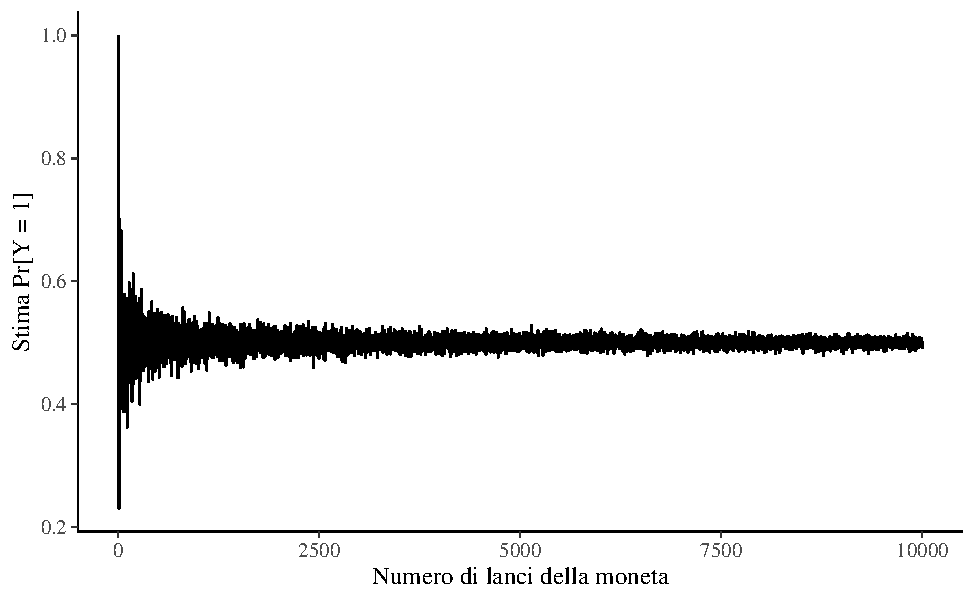
\includegraphics{ds4psy_files/figure-latex/legge-grandi-n-1-1} 

}

\caption{Stima della probabilità di successo in funzione del numero di lanci di una moneta.}\label{fig:legge-grandi-n-1}
\end{figure}

Dato che il grafico \ref{fig:legge-grandi-n-1} espresso su una scala lineare non rivela chiaramente l'andamento della simulazione, possiamo usare un grafico che impone una scala logaritmica sull'asse delle ascisse (\(x\)). Su scala logaritmica, i valori tra 1 e 10 vengono tracciati all'incirca con la stessa ampiezza che si osseerva per valori tra 50 e 700, eccetera.

\begin{Shaded}
\begin{Highlighting}[]
\NormalTok{d }\SpecialCharTok{\%\textgreater{}\%}
  \FunctionTok{ggplot}\NormalTok{(}
    \FunctionTok{aes}\NormalTok{(}\AttributeTok{x =}\NormalTok{ n, }\AttributeTok{y =}\NormalTok{ estimate)}
\NormalTok{  ) }\SpecialCharTok{+}
  \FunctionTok{geom\_line}\NormalTok{() }\SpecialCharTok{+}
  \FunctionTok{scale\_x\_log10}\NormalTok{(}
    \AttributeTok{breaks =} \FunctionTok{c}\NormalTok{(}
      \DecValTok{1}\NormalTok{, }\DecValTok{3}\NormalTok{, }\DecValTok{10}\NormalTok{, }\DecValTok{50}\NormalTok{, }\DecValTok{200}\NormalTok{,}
      \DecValTok{700}\NormalTok{, }\DecValTok{2500}\NormalTok{, }\DecValTok{10000}
\NormalTok{    )}
\NormalTok{  ) }\SpecialCharTok{+}
  \FunctionTok{theme}\NormalTok{(}\AttributeTok{legend.title =} \FunctionTok{element\_blank}\NormalTok{()) }\SpecialCharTok{+}
  \FunctionTok{labs}\NormalTok{(}
    \AttributeTok{x =} \StringTok{"Numero di lanci della moneta"}\NormalTok{,}
    \AttributeTok{y =} \StringTok{"Stima Pr[Y = 1]"}
\NormalTok{  )}
\end{Highlighting}
\end{Shaded}

\begin{figure}[h]

{\centering 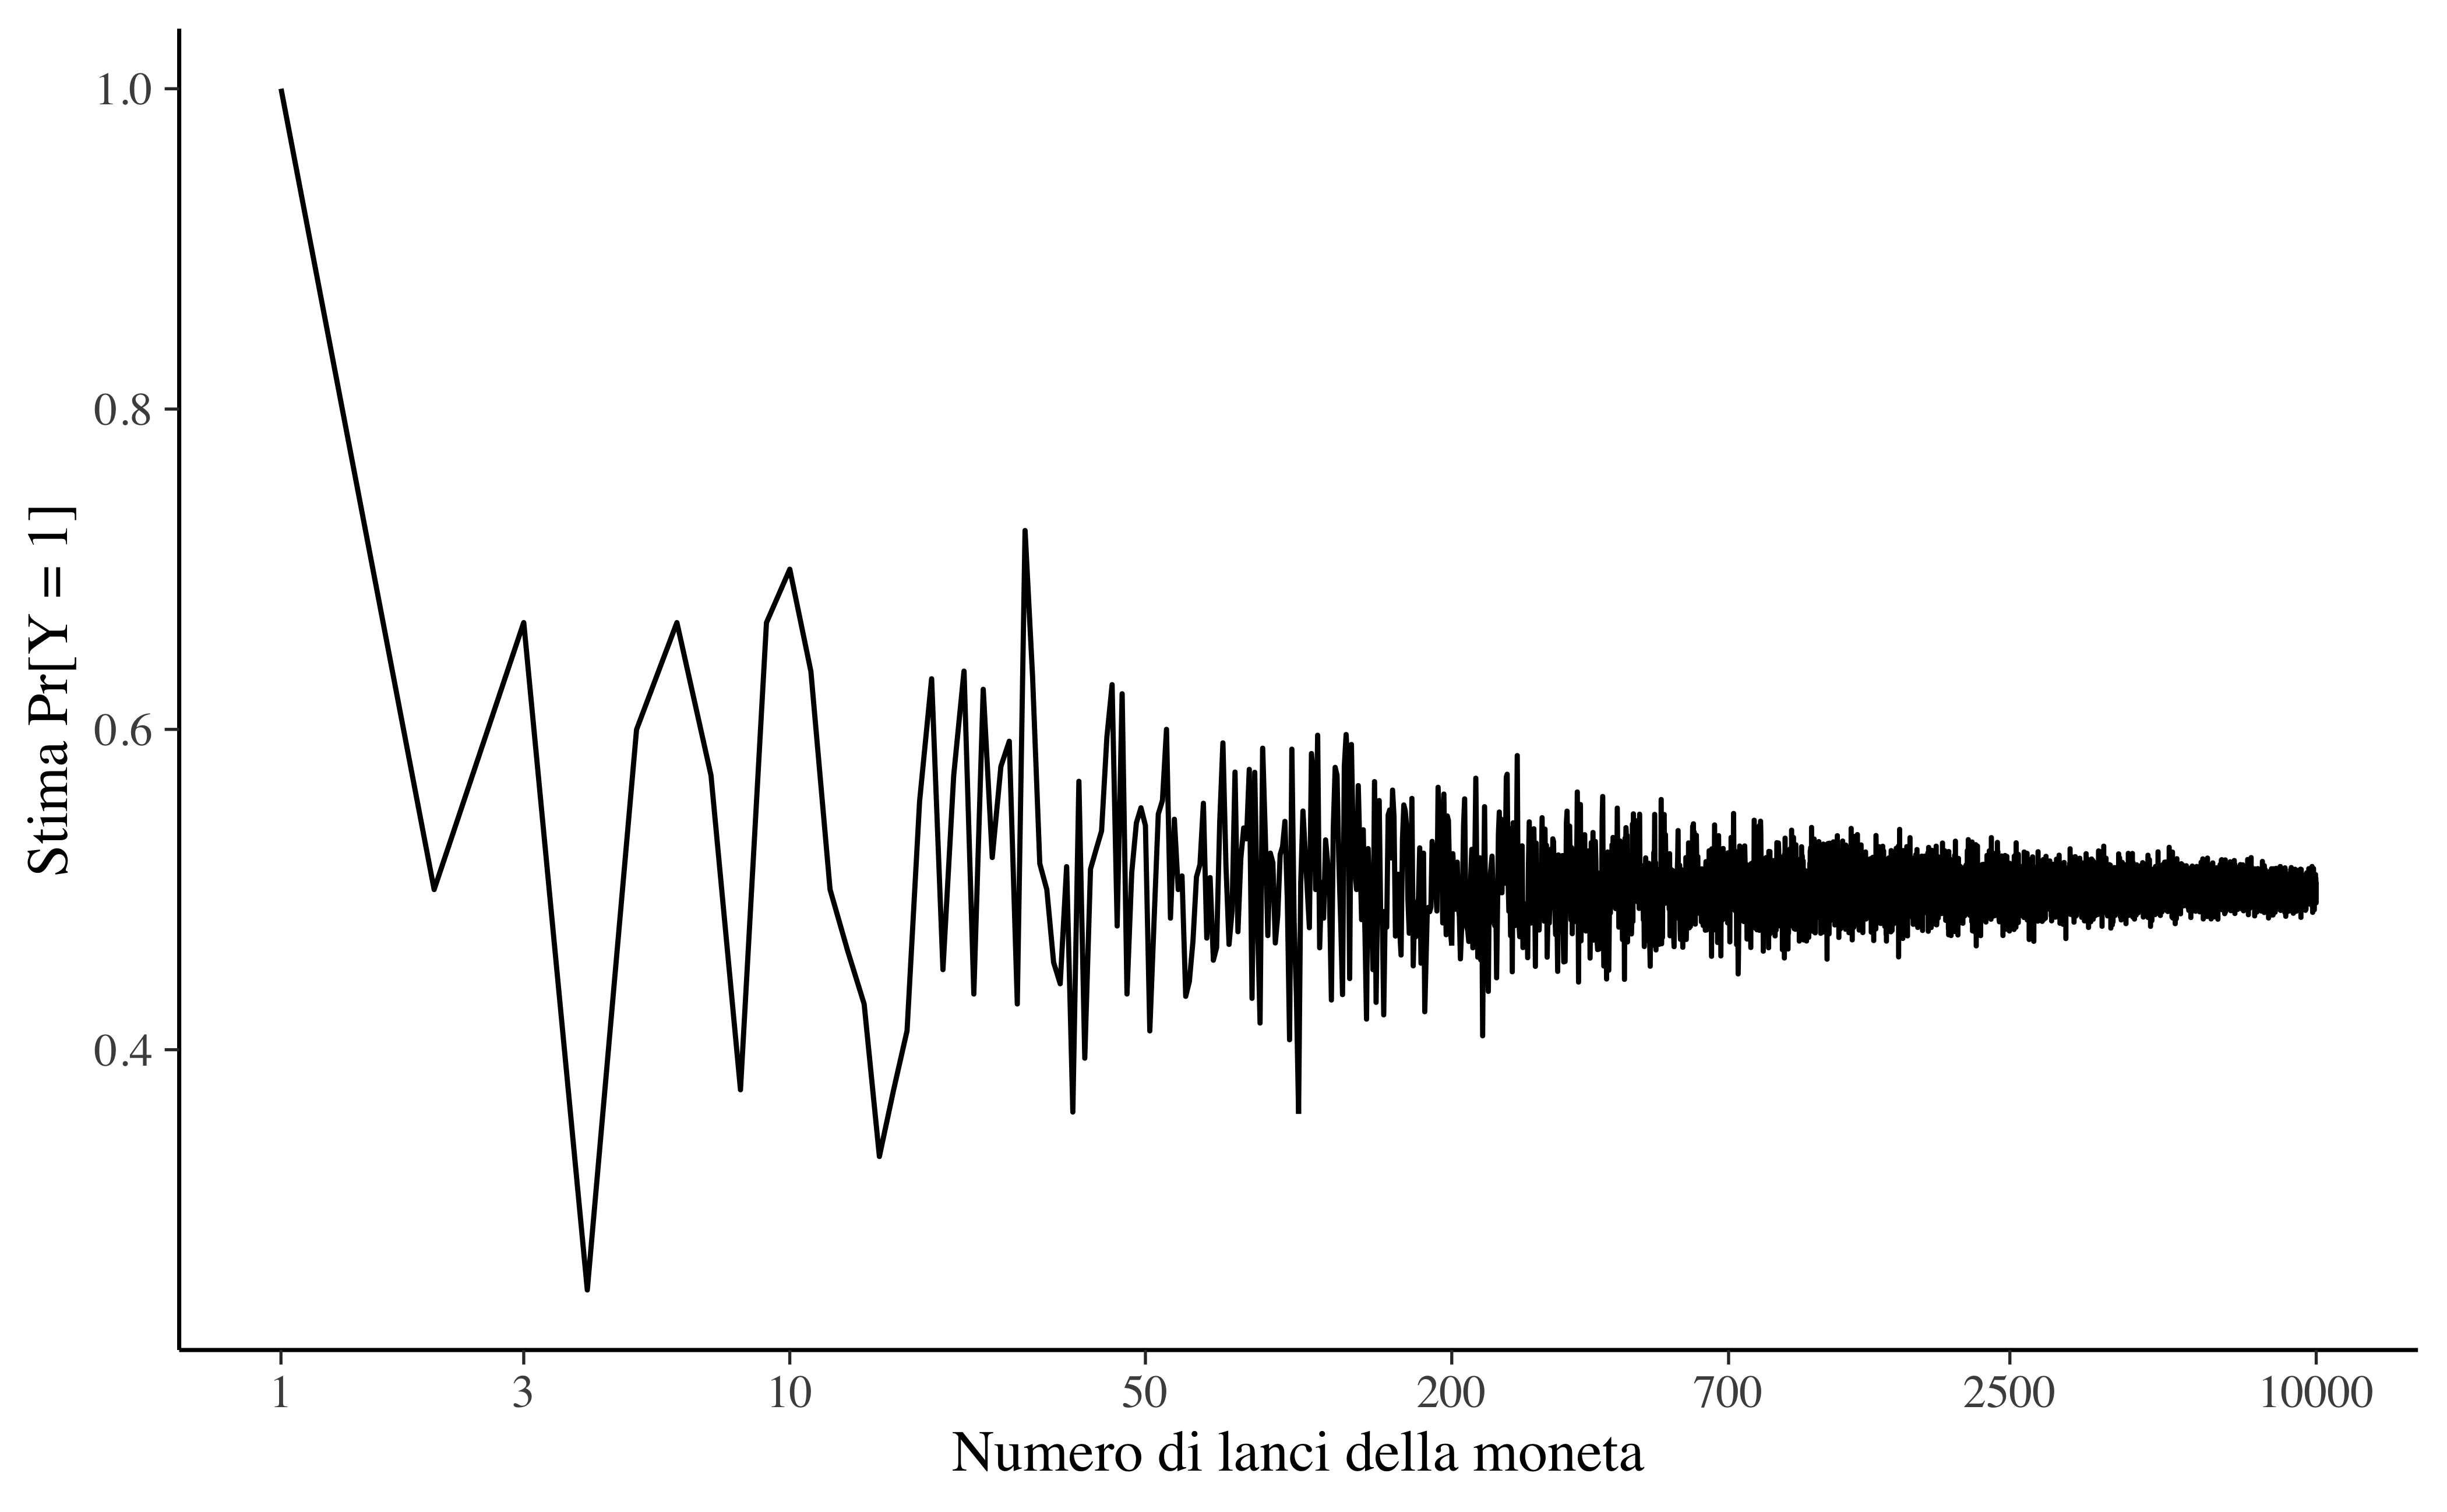
\includegraphics{ds4psy_files/figure-latex/legge-grandi-n-2-1} 

}

\caption{Stima della probabilità di successo in funzione del numero di lanci di una moneta -- scala logaritmica.}\label{fig:legge-grandi-n-2}
\end{figure}

La \emph{legge dei grandi numeri} ci dice che, all'aumentare del numero di ripetizioni dell'esperimento casuale, la media dei risultati ottenuti tenderà ad avvicinarsi al valore atteso, man mano che verranno eseguite più prove. Nel caso presente, la figura \ref{fig:legge-grandi-n-2} mostra appunto che, all'aumentare del numero \emph{M} di lanci della moneta, la stima di \(Pr[Y = 1]\) tende a convergere al vero valore di 0.5.

\hypertarget{variabili-casuali-multiple}{%
\section{Variabili casuali multiple}\label{variabili-casuali-multiple}}

Le variabili casuali non esistono isolatamente. Abbiamo iniziato con una singola variabile casuale \emph{Y} che rappresenta il risultato di un singolo, specifico lancio di una moneta equlibrata. Ma supponiamo ora di lanciare la moneta tre volte. Ciò suggerisce che i risultati di ciascuno dei tre lanci possono essere rappresentati da una diversa variabile casuale, ad esepio, \(Y_1 , Y_2 , Y_3\). Possiamo assumere che ogni lancio sia indipendente, ovvero che non dipenda dal risultato degli altri lanci. Ognuna di queste variabili \(Y_n\) per \(n \in 1:3\) ha \(Pr[Y_n =1]=0.5\) e \(Pr[Y_n =0]=0.5\).

È possibile combinare più variabili casuali usando le operazioni aritmetiche. Se \(Y_1 , Y_2, Y_3\) sono variabili casuali che rappresentano tre lanci di una moneta equilibrata (o un lancio di tre monete equilibrate), possiamo definire la somma di tali variabili casuali come

\[
Z = Y_1 + Y_2 + Y_3.
\]

Possiamo simulare i valori assunti dalla variabile casuale \emph{Z} simulando i valori di \(Y_1, Y_2, Y_3\) per poi sommarli.

\begin{Shaded}
\begin{Highlighting}[]
\NormalTok{y1 }\OtherTok{\textless{}{-}} \FunctionTok{rbinom}\NormalTok{(}\DecValTok{1}\NormalTok{, }\DecValTok{1}\NormalTok{, }\FloatTok{0.5}\NormalTok{)}
\NormalTok{y2 }\OtherTok{\textless{}{-}} \FunctionTok{rbinom}\NormalTok{(}\DecValTok{1}\NormalTok{, }\DecValTok{1}\NormalTok{, }\FloatTok{0.5}\NormalTok{)}
\NormalTok{y3 }\OtherTok{\textless{}{-}} \FunctionTok{rbinom}\NormalTok{(}\DecValTok{1}\NormalTok{, }\DecValTok{1}\NormalTok{, }\FloatTok{0.5}\NormalTok{)}
\FunctionTok{c}\NormalTok{(y1, y2, y3)}
\CommentTok{\#\textgreater{} [1] 1 0 1}
\NormalTok{z }\OtherTok{\textless{}{-}} \FunctionTok{sum}\NormalTok{(}\FunctionTok{c}\NormalTok{(y1, y2, y3))}
\FunctionTok{cat}\NormalTok{(}\StringTok{"z ="}\NormalTok{, z, }\StringTok{"}\SpecialCharTok{\textbackslash{}n}\StringTok{"}\NormalTok{)}
\CommentTok{\#\textgreater{} z = 2}
\end{Highlighting}
\end{Shaded}

ovvero,

\begin{Shaded}
\begin{Highlighting}[]
\NormalTok{y }\OtherTok{\textless{}{-}} \FunctionTok{rep}\NormalTok{(}\ConstantTok{NA}\NormalTok{, }\DecValTok{3}\NormalTok{)}
\ControlFlowTok{for}\NormalTok{ (i }\ControlFlowTok{in} \DecValTok{1}\SpecialCharTok{:}\DecValTok{3}\NormalTok{) \{}
\NormalTok{  y[i] }\OtherTok{\textless{}{-}} \FunctionTok{rbinom}\NormalTok{(}\DecValTok{1}\NormalTok{, }\DecValTok{1}\NormalTok{, }\FloatTok{0.5}\NormalTok{)}
\NormalTok{\}}
\NormalTok{y}
\CommentTok{\#\textgreater{} [1] 0 1 1}
\NormalTok{z }\OtherTok{\textless{}{-}} \FunctionTok{sum}\NormalTok{(y)}
\FunctionTok{cat}\NormalTok{(}\StringTok{"z ="}\NormalTok{, z, }\StringTok{"}\SpecialCharTok{\textbackslash{}n}\StringTok{"}\NormalTok{)}
\CommentTok{\#\textgreater{} z = 2}
\end{Highlighting}
\end{Shaded}

oppure, ancora più semplicemente:

\begin{Shaded}
\begin{Highlighting}[]
\NormalTok{y }\OtherTok{\textless{}{-}} \FunctionTok{rbinom}\NormalTok{(}\DecValTok{3}\NormalTok{, }\DecValTok{1}\NormalTok{, }\FloatTok{0.5}\NormalTok{)}
\NormalTok{y}
\CommentTok{\#\textgreater{} [1] 1 0 1}
\NormalTok{z }\OtherTok{\textless{}{-}} \FunctionTok{sum}\NormalTok{(y)}
\FunctionTok{cat}\NormalTok{(}\StringTok{"z ="}\NormalTok{, z, }\StringTok{"}\SpecialCharTok{\textbackslash{}n}\StringTok{"}\NormalTok{)}
\CommentTok{\#\textgreater{} z = 2}
\end{Highlighting}
\end{Shaded}

Possiamo ripetere questa simulazione \(M = 1e5\) volte:

\begin{Shaded}
\begin{Highlighting}[]
\NormalTok{M }\OtherTok{\textless{}{-}} \FloatTok{1e5}
\NormalTok{z }\OtherTok{\textless{}{-}} \FunctionTok{rep}\NormalTok{(}\ConstantTok{NA}\NormalTok{, M)}
\ControlFlowTok{for}\NormalTok{ (i }\ControlFlowTok{in} \DecValTok{1}\SpecialCharTok{:}\NormalTok{M) \{}
\NormalTok{  y }\OtherTok{\textless{}{-}} \FunctionTok{rbinom}\NormalTok{(}\DecValTok{3}\NormalTok{, }\DecValTok{1}\NormalTok{, }\FloatTok{0.5}\NormalTok{)}
\NormalTok{  z[i] }\OtherTok{\textless{}{-}} \FunctionTok{sum}\NormalTok{(y)}
\NormalTok{\}}
\end{Highlighting}
\end{Shaded}

e calcolare una stima della probabilità che la variabile casuale \(Z\) assuma i valori 0, 1, 2, 3:

\begin{Shaded}
\begin{Highlighting}[]
\FunctionTok{table}\NormalTok{(z) }\SpecialCharTok{/}\NormalTok{ M}
\CommentTok{\#\textgreater{} z}
\CommentTok{\#\textgreater{}      0      1      2      3 }
\CommentTok{\#\textgreater{} 0.1258 0.3750 0.3748 0.1244}
\end{Highlighting}
\end{Shaded}

Nel caso di 4 monete equilibrate, avremo:

\begin{Shaded}
\begin{Highlighting}[]
\NormalTok{M }\OtherTok{\textless{}{-}} \FloatTok{1e5}
\NormalTok{z }\OtherTok{\textless{}{-}} \FunctionTok{rep}\NormalTok{(}\ConstantTok{NA}\NormalTok{, M)}
\ControlFlowTok{for}\NormalTok{ (i }\ControlFlowTok{in} \DecValTok{1}\SpecialCharTok{:}\NormalTok{M) \{}
\NormalTok{  y }\OtherTok{\textless{}{-}} \FunctionTok{rbinom}\NormalTok{(}\DecValTok{4}\NormalTok{, }\DecValTok{1}\NormalTok{, }\FloatTok{0.5}\NormalTok{)}
\NormalTok{  z[i] }\OtherTok{\textless{}{-}} \FunctionTok{sum}\NormalTok{(y)}
\NormalTok{\}}
\FunctionTok{table}\NormalTok{(z) }\SpecialCharTok{/}\NormalTok{ M}
\CommentTok{\#\textgreater{} z}
\CommentTok{\#\textgreater{}       0       1       2       3       4 }
\CommentTok{\#\textgreater{} 0.06340 0.24917 0.37360 0.25022 0.06361}
\end{Highlighting}
\end{Shaded}

Una variabile casuale le cui modalità possono essere costituite solo da numeri interi è detta \emph{variabile casuale discreta}:

\[
\mathbb{Z} = \dots, -2, -1, 0, 1, 2, \dots
\]

\hypertarget{sec:fun-mass-prob}{%
\section{Funzione di massa di probabilità}\label{sec:fun-mass-prob}}

È conveniente avere una funzione che associa ogni possibile valore di una variabile casuale alla sua probabilità. In generale, ciò è possibile se e solo se la variabile casuale è discreta, così com'è stata definita nel Paragrafo precedente.

Ad esempio, se consideriamo \(Z = Y_1 + \dots + Y_4\) come il numero di risultati ``testa'' in 4 lanci della moneta, allora possiamo definire la seguente funzione:

\[
\begin{array}{rclll}
p_Z(0) & = & 1/16 & & \mathrm{TTTT}
\\
p_Z(1) & = & 4/16 & & \mathrm{HTTT, THTT, TTHT, TTTH}
\\
p_Z(2) & = & 6/16 & & \mathrm{HHTT, HTHT, HTTH, THHT, THTH, TTTH}
\\
p_Z(3) & = & 4/16 & & \mathrm{HHHT, HHTH, HTHH, THHH}
\\
p_Z(4) & = & 1/16 & & \mathrm{HHHH}
\end{array}
\]

Il lancio di quattro monete può produrre sedici possibili risultati. Dato che i lanci sono indipendenti e le monete sono equilibrate, ogni possibile risultato è ugualmente probabile. Nella tabella in alto, le sequenze dei risultati possibili del lancio delle 4 monete sono riportate nella colonna più a destra. Le probabilità si ottengono dividendo il numero di sequenze che producono lo stesso numero di eventi testa per il numero dei risultati possibili.

La funzione \(p_Z\) è stata costruita per mappare un valore \(u\) per \(Z\) alla probabilità dell'evento \(Z = u\). Convenzionalmente, queste probabilità sono scritte come

\[
p_Z(z) = \mbox{Pr}[Z = z].
\]

La parte a destra dell'uguale si può leggere come: ``la probabilità che la variabile casuale \(Z\) assuma il valore \(z\)''.

Una funzione definita come sopra è detta \emph{funzione di massa di probabilità} della variabile casuale \(Z\). Ad ogni variabile casuale discreta è associata un'unica funzione di massa di probabilità.

Una rappresentazione grafica della stima della funzione di massa di probabilità per l'esperimento casuale del lancio di quattro monete equilibrate è fornita nella figura \ref{fig:barplot-mdf-4coins}.

\begin{Shaded}
\begin{Highlighting}[]
\FunctionTok{set.seed}\NormalTok{(}\DecValTok{1234}\NormalTok{)}
\NormalTok{M }\OtherTok{\textless{}{-}} \FloatTok{1e5}
\NormalTok{nflips }\OtherTok{\textless{}{-}} \DecValTok{4}
\NormalTok{u }\OtherTok{\textless{}{-}} \FunctionTok{rbinom}\NormalTok{(M, nflips, }\FloatTok{0.5}\NormalTok{)}
\NormalTok{x }\OtherTok{\textless{}{-}} \DecValTok{0}\SpecialCharTok{:}\NormalTok{nflips}
\NormalTok{y }\OtherTok{\textless{}{-}} \FunctionTok{rep}\NormalTok{(}\ConstantTok{NA}\NormalTok{, nflips }\SpecialCharTok{+} \DecValTok{1}\NormalTok{)}
\ControlFlowTok{for}\NormalTok{ (n }\ControlFlowTok{in} \DecValTok{0}\SpecialCharTok{:}\NormalTok{nflips) \{}
\NormalTok{  y[n }\SpecialCharTok{+} \DecValTok{1}\NormalTok{] }\OtherTok{\textless{}{-}} \FunctionTok{sum}\NormalTok{(u }\SpecialCharTok{==}\NormalTok{ n) }\SpecialCharTok{/}\NormalTok{ M}
\NormalTok{\}}
\NormalTok{bar\_plot }\OtherTok{\textless{}{-}}
  \FunctionTok{data.frame}\NormalTok{(}\AttributeTok{Z =}\NormalTok{ x, }\AttributeTok{count =}\NormalTok{ y) }\SpecialCharTok{\%\textgreater{}\%}
  \FunctionTok{ggplot}\NormalTok{(}
    \FunctionTok{aes}\NormalTok{(}\AttributeTok{x =}\NormalTok{ Z, }\AttributeTok{y =}\NormalTok{ count)}
\NormalTok{  ) }\SpecialCharTok{+}
  \FunctionTok{geom\_bar}\NormalTok{(}\AttributeTok{stat =} \StringTok{"identity"}\NormalTok{) }\SpecialCharTok{+}
  \FunctionTok{scale\_x\_continuous}\NormalTok{(}
    \AttributeTok{breaks =} \DecValTok{0}\SpecialCharTok{:}\DecValTok{4}\NormalTok{,}
    \AttributeTok{labels =} \FunctionTok{c}\NormalTok{(}\DecValTok{0}\NormalTok{, }\DecValTok{1}\NormalTok{, }\DecValTok{2}\NormalTok{, }\DecValTok{3}\NormalTok{, }\DecValTok{4}\NormalTok{)}
\NormalTok{  ) }\SpecialCharTok{+}
  \FunctionTok{labs}\NormalTok{(}
    \AttributeTok{y =} \StringTok{"Probabilità stimata Pr[Z = z]"}
\NormalTok{  )}
\NormalTok{bar\_plot}
\end{Highlighting}
\end{Shaded}

\begin{figure}[h]

{\centering 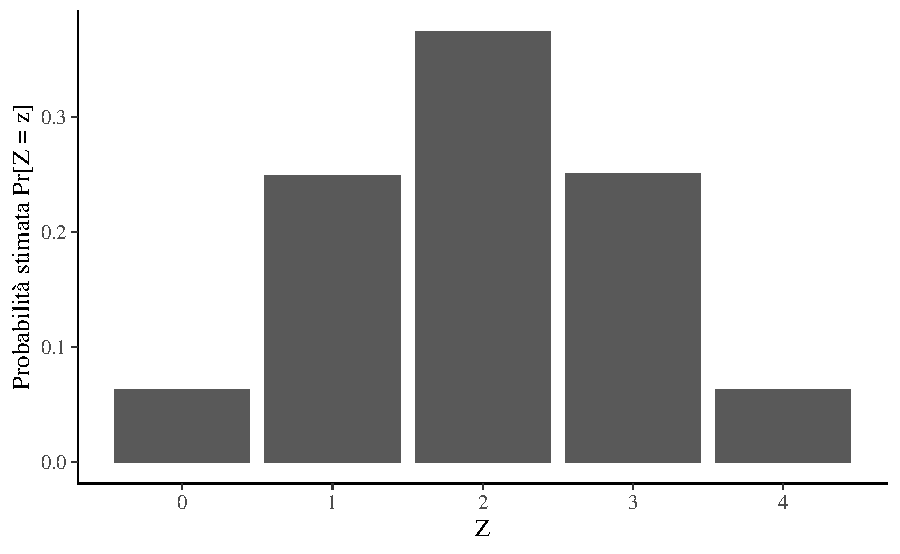
\includegraphics{ds4psy_files/figure-latex/barplot-mdf-4coins-1} 

}

\caption{Grafico di $M = 100\,000$ simulazioni della funzione di massa di probabilità di una variabile casuale definita come il numero di teste in quattro lanci di una moneta equilibrata.}\label{fig:barplot-mdf-4coins}
\end{figure}

Se \(A\) è un sottoinsieme della variabile casuale \(Z\), allora denotiamo con \(P_{z}(A)\) la probabilità assegnata ad \(A\) dalla distribuzione \(P_{z}\). Mediante una distribuzione di probabilità \(P_{z}\) è dunque possibile determinare la probabilità di ciascun sottoinsieme \(A \subset Z\) come

\[
P_{z}(A) = \sum_{z \in A} P_{z}(Z).
\]

\begin{example}
Nel caso dell'esempio discusso nella Sezione \ref{sec:fun-mass-prob}, la probabilità che la variabile casuale \(Z\) sia un numero dispari è

\[
Pr(\text{Z è un numero dispari}) = P_{z}(Z = 1) + P_{z}(Z = 3) = \frac{4}{16} + \frac{4}{16} = \frac{1}{2}.
\]
\end{example}

\hypertarget{commenti-e-considerazioni-finali}{%
\section*{Commenti e considerazioni finali}\label{commenti-e-considerazioni-finali}}


In questo capitolo abbiamo visto come si costruisce lo spazio campionario di un esperimento casuale, quali sono le proprietà di base della probabilità e come si assegnano le probabilità agli eventi definiti sopra uno spazio campionario discreto. Abbiamo anche introdotto le nozioni di ``variabile casuale'', ovvero di una variabile che prende i suoi valori casualmente. E abbiamo descritto il modo di specificare la probabilità con cui sono presi i differenti valori, ovvero la funzione di distribuzione probabilistica \(F(X) = Pr(X < x)\), e la funzione di massa di probabilità. Le procedure di analisi dei dati psicologici che discuteremo in seguito faranno un grande uso di questi concetti e della notazione qui introdotta.

\hypertarget{chapter-prob-cond}{%
\chapter{Probabilità condizionata}\label{chapter-prob-cond}}

Il fondamento della statistica bayesiana è il teorema di Bayes e il fondamento del teorema di Bayes è la probabilità condizionata. In questo Capitolo, inizieremo a presentare la probabilità condizionata. Nel Capitolo successivo, partendo dalla definizione di probabilità condizionata, deriveremo il teorema di Bayes.

\hypertarget{sec:bayes-cancer}{%
\section{Probabilità condizionata su altri eventi}\label{sec:bayes-cancer}}

L'attribuzione di una probabilità ad un evento è sempre condizionata dalle conoscenze che abbiamo a disposizione. Per un determinato stato di conoscenze, attribuiamo ad un dato evento una certa probabilità di verificarsi; ma se il nostro stato di conoscenze cambia, allora cambierà anche la probabilità che attribuiremo all'evento in questione. Infatti, si può pensare che tutte le probabilità siano probabilità condizionate, anche se l'evento condizionante non è sempre esplicitamente menzionato. Consideriamo il seguente problema.

\begin{exercise}

Supponiamo che lo screening per la diagnosi precoce del tumore mammario si avvalga di test che sono accurati al 90\%, nel senso che il 90\% delle donne con cancro e il 90\% delle donne senza cancro saranno classificate correttamente. Supponiamo che l'1\% delle donne sottoposte allo screening abbia effettivamente il cancro al seno. Ci chiediamo: qual è la probabilità che una donna scelta casualmente abbia una mammografia positiva e, se ce l'ha, qual è la probabilità che abbia davvero il cancro?

Per risolvere questo problema, supponiamo che il test in questione venga somministrato ad un grande campione di donne, diciamo a 1000 donne. Di queste 1000 donne, 10 (ovvero, l'1\%) hanno il cancro al seno. Per queste 10 donne, il test darà un risultato positivo in 9 casi (ovvero, nel 90\% dei casi). Per le rimanenti 990 donne che non hanno il cancro al seno, il test darà un risultato positivo in 99 casi (se la probabilità di un vero positivo è del 90\%, la probabilità di un falso positivo è del 10\%). Questa situazione è rappresentata nella figura \ref{fig:mammografia}.

Combinando i due risultati precedenti, vediamo che il test dà un risultato positivo per 9 donne che hanno effettivamente il cancro al seno e per 99 donne che non ce l'hanno, per un totale di 108 risultati positivi. Dunque, la probabilità di ottenere un risultato positivo al test è \(\frac{108}{1000}\) = 11\%. Ma delle 108 donne che hanno ottenuto un risultato positivo al test, solo 9 hanno il cancro al seno. Dunque, la probabilità di avere il cancro, dato un risultato positivo al test, è pari a \(\frac{9}{108}\) = 8\%.

\begin{figure}[h]

{\centering 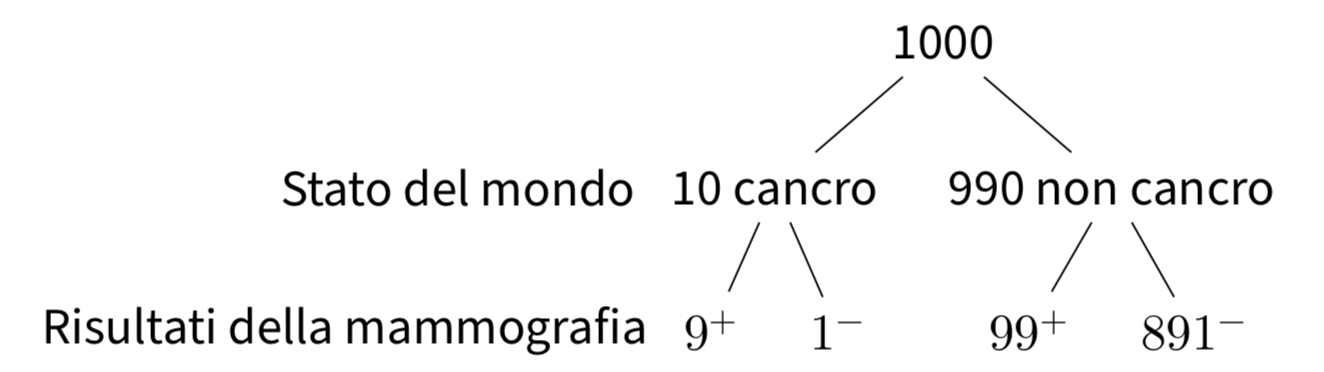
\includegraphics[width=0.67\linewidth]{images/mammografia} 

}

\caption{Rappresentazione ad albero che riporta le frequenze attese dei risultati di una mammografia in un campione di 1,000 donne.}\label{fig:mammografia}
\end{figure}

\end{exercise}

Nell'esercizio precedente, la probabilità dell'evento ``ottenere un risultato positivo al test'' è una probabilità non condizionata, mentre la probabilità dell'evento ``avere il cancro al seno, dato che il test ha prodotto un risultato positivo'' è una probabilità condizionata. In termini generali, la probabilità condizionata \(P(A \mid B)\) rappresenta la probabilità che si verifichi l'evento \(A\) sapendo che si è verificato l'evento \(B\) (oppure: la probabilità di \(A\) in una prova valida solo se si verifica anche \(B\)). Ciò ci conduce alla seguente definizione.

\begin{definition}
Dato un qualsiasi evento \(A\), si chiama \emph{probabilità condizionata} di \(A\) dato \(B\) il numero

\begin{equation}
P(A \mid B) = \frac{P(A \cap B)}{P(B)}, \quad \text{con}\, P(B) > 0,
\label{eq:probcond}
\end{equation}

dove \(P(A\cap B)\) è la probabilità congiunta dei due eventi, ovvero la probabilità che si verifichino entrambi.
\end{definition}

Nella \eqref{eq:probcond} possiamo distinguere tra la probabilità congiunta \(P(A \cap B)\), la probabilità condizionata \(P(A \mid B)\) e la probabilità marginale \(P(B)\).

\begin{exercise}
Da un mazzo di 52 carte (13 carte per ciascuno dei 4 semi) ne viene estratta una in modo casuale. Qual è la probabilità che esca una figura di cuori? Sapendo che la carta estratta ha il seme di cuori, qual è la probabilità che il valore numerico della carta sia 7, 8 o 9?

Ci sono 13 carte di cuori, dunque la risposta alla prima domanda è 1/4. Per rispondere alla seconda domanda consideriamo solo le 13 carte di cuori; la probabilità cercata è dunque 3/13.
\end{exercise}

\hypertarget{la-fallacia-del-condizionale-trasposto}{%
\subsection{La fallacia del condizionale trasposto}\label{la-fallacia-del-condizionale-trasposto}}

Un errore comune che si commette è quello di credere che \(P(A \mid B)\) sia uguale a \(P(B \mid A)\). Tale fallacia ha particolare risalto in ambito forense tanto che è conosciuta con il nome di ``fallacia del procuratore''. In essa, una piccola probabilità dell'evidenza, data l'innocenza, viene erroneamente interpretata come la probabilità dell'innocenza, data l'evidenza.

Consideriamo il caso di un esame del DNA. Un esperto forense potrebbe affermare, ad esempio, che ``se l'imputato è innocente, c'è solo una possibilità su un miliardo che vi sia una corrispondenza tra il suo DNA e il DNA trovato sulla scena del crimine''. Ma talvolta questa probabilità è erroneamente interpretata come avesse il seguente significato: ``date le prove del DNA, c'è solo una possibilità su un miliardo che l'imputato sia innocente''.

Le considerazioni precedenti risultano più chiare se facciamo nuovamente riferimento all'esercizio sul tumore mammario descritto sopra. In tale esercizio abbiamo visto come la probabilità di cancro dato un risultato positivo al test sia uguale a 0.08. Tale probabilità è molto diversa dalla probabilità di un risultato positivo al test data la presenza del cancro. Infatti, questa seconda probabilità è uguale a 0.90 ed è descritta nel problema come una delle caratteristiche del test in questione.

\hypertarget{legge-delle-probabilituxe0-composte}{%
\section{Legge delle probabilità composte}\label{legge-delle-probabilituxe0-composte}}

Dalla definizione di probabilità condizionata è possibile esprimere la probabilità congiunta come prodotto di due probabilità, una condizionata e una marginale. La legge delle probabilità composte afferma che la probabilità che si verifichino due eventi \(A\) e \(B\) è pari alla probabilità di uno dei due eventi moltiplicato con la probabilità dell'altro evento condizionato al verificarsi del primo. Per esempio se conosciamo la probabilità marginale \(P(B)\) e la probabilità condizionata \(P(A \mid B)\) otteniamo

\begin{equation}
P(A \cap B) = P(B)P(A \mid B),
\label{eq:probcondinv}
\end{equation}

mentre se conosciamo la probabilità marginale \(P(A)\) e la probabilità condizionata \(P(B \mid A)\) otteniamo

\[
P(A \cap B) = P(A)P(B \mid A).
\]

L'equazione \eqref{eq:probcondinv} si estende al caso di \(n\) eventi \(A_1, \dots, A_n\) nella forma seguente:

\begin{equation}
P\left( \bigcap_{k=1}^n A_k \right) = \prod_{k=1}^n \left(  A_k  \ \Biggl\lvert \ \bigcap_{j=1}^{k-1} A_j \right)
\label{eq:probcomposte}
\end{equation}

Per esempio, nel caso di quattro eventi abbiamo

\begin{equation}
\begin{split}
P(A_1 \cap A_2 \cap A_3 \cap A_4) = {}& P(A_1) \cdot P(A_2 \mid A_1) \cdot  P(A_3 \mid A_1 \cap A_2) \cdot \\
 & P(A_4 \mid A_1 \cap A_2 \cap A_{3}).\notag
\end{split}
\end{equation}

\begin{exercise}
Da un'urna contenente 6 palline bianche e 4 nere si estrae una pallina per volta, senza reintrodurla nell'urna. Indichiamo con \(B_i\) l'evento: ``esce una pallina bianca alla \(i\)-esima estrazione'' e con \(N_i\) l'estrazione di una pallina nera. L'evento: ``escono due palline bianche nelle prime due estrazioni'' è rappresentato dalla intersezione \(\{B_1 \cap B_2\}\) e la sua probabilità vale, per la \eqref{eq:probcondinv}

\[
P(B_1 \cap B_2) = P(B_1)P(B_2 \mid B_1).
\]

\(P(B_1)\) vale 6/10, perché nella prima estrazione \(\Omega\) è costituito da 10 elementi: 6 palline bianche e 4 nere. La probabilità condizionata \(P(B_2 \mid B_1)\) vale 5/9, perché nella seconda estrazione, se è verificato l'evento \(B_1\), lo spazio campionario consiste di 5 palline bianche e 4 nere. Si ricava pertanto:

\[
P(B_1 \cap B_2) = \frac{6}{10} \cdot \frac{5}{9} = \frac{1}{3}.
\]

In modo analogo si ha che

\[
P(N_1 \cap N_2) = P(N_1)P(N_2 \mid N_1) = \frac{4}{10} \cdot \frac{3}{9} = \frac{4}{30}.
\]

Se l'esperimento consiste nell'estrazione successiva di 3 palline, la probabilità che queste siano tutte bianche vale, per la \eqref{eq:probcomposte}:

\[
P(B_1 \cap B_2 \cap B_3)=P(B_1)P(B_2 \mid B_1)P(B_3 \mid B_1 \cap B_2),
\]

dove la probabilità \(P(B_3 \mid B_1 \cap B_2)\) si calcola supponendo che si sia verificato l'evento condizionante \(\{B_1 \cap B_2\}\). Lo spazio campionario per questa probabilità condizionata è costituito da 4 palline bianche e 4 nere, per cui \(P(B_3 \mid B_1 \cap B_2) = 1/2\) e quindi:

\[
P (B_1 \cap B_2 \cap B_3) = \frac{6}{10}\cdot\frac{5}{9} \cdot\frac{4}{8}  = \frac{1}{6}.
\]

La probabilità dell'estrazione di tre palline nere è invece:

\[
\begin{aligned}
P(N_1 \cap N_2 \cap N_3) &= P(N_1)P(N_2 \mid N_1)P(N_3 \mid N_1 \cap N_2)\notag\\ 
&= \frac{4}{10} \cdot \frac{3}{9} \cdot \frac{2}{8} = \frac{1}{30}.\notag
\end{aligned}
\]
\end{exercise}

\hypertarget{lindipendendenza-stocastica}{%
\section{L'indipendendenza stocastica}\label{lindipendendenza-stocastica}}

Un concetto molto importante per le applicazioni statistiche della probabilità è quello dell'indipendenza stocastica. La definizione \eqref{eq:probcond} esprime il concetto intuitivo di indipendenza di un evento da un altro, nel senso che il verificarsi di \(A\) non influisce sulla probabilità del verificarsi di \(B\), ovvero non la condiziona. Infatti, per la definizione \eqref{eq:probcond} di probabilità condizionata, si ha che, se \(A\) e \(B\) sono due eventi indipendenti, risulta:

\[
P(A \mid B) = \frac{P(A)P(B)}{P(B)} = P(A).\notag
\]

Possiamo dunque dire che due eventi \(A\) e \(B\) sono indipendenti se

\begin{equation}
\begin{split}
P(A \mid B) &= P(A), \\
P(B \mid A) &= P(B).
\end{split}
\end{equation}

Si noti inoltre che, se due eventi con probabilità non nulla sono statisticamente indipendenti, la legge delle probabilità totali espressa dalla \eqref{eq:probunione} \begin{equation}
P(A \cup B) = P(A) + P(B) - P(A \cap B)
\label{eq:probunione}
\end{equation}

si modifica nella relazione seguente:

\begin{equation}
P(A \cup B) = P(A) + P(B) - P(A)P(B).
\end{equation}

\begin{exercise}
Nel lancio di due dadi non truccati, si considerino gli eventi: \emph{A} = \{esce un 1 o un 2 nel primo lancio\} e \emph{B} = \{il punteggio totale è 8\}. Gli eventi \emph{A} e \emph{B} sono indipendenti?

Rappresentiamo qui sotto lo spazio campionario dell'esperimento casuale.

\begin{figure}[h]

{\centering 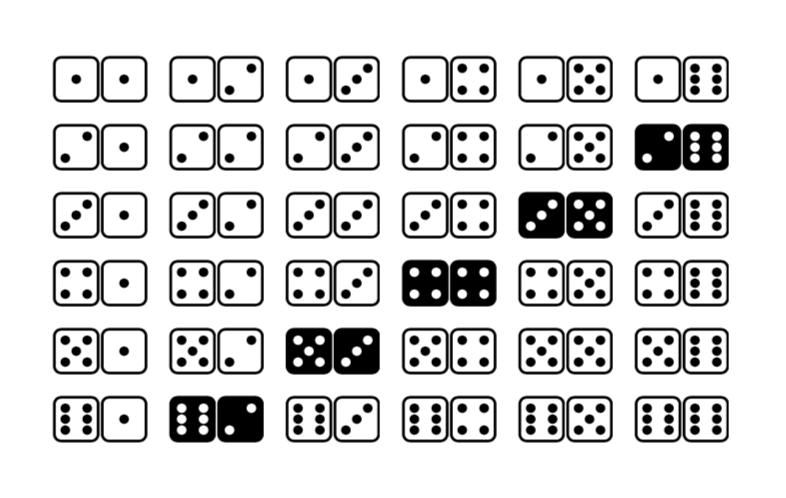
\includegraphics[width=0.7\linewidth]{images/sampling-space-dice} 

}

\caption{Rappresentazione dello spazio campionario dei risultati dell'esperimento casuale corrispondente al lancio di due dadi bilanciati. Sono evidenziati gli eventi elementari che costituiscono l'evento A: esce un 1 o un 2 nel primo lancio.}\label{fig:sampling-space-dice}
\end{figure}

Gli eventi \emph{A} e \emph{B} non sono statisticamente indipendenti. Infatti, le loro probabilità valgono \emph{P}(A) = 12/36 e \emph{P}(B) = 5/36 e la probabilità della loro intersezione è

\[
P(A \cap B) = 1/36 = 3/108 \neq P(A)P(B) = 5/108.
\]
\end{exercise}

\begin{remark}
Il concetto di indipendenza è del tutto differente da quello di incompatibilità. Si noti infatti che due eventi \emph{A} e \emph{B} incompatibili (per i quali si ha \(A \cap B = \emptyset\)) sono statisticamente dipendenti, poiché il verificarsi dell'uno esclude il verificarsi dell'altro: \(P(A \cap B)=0 \neq P(A)P(B)\).
\end{remark}

\hypertarget{commenti-e-considerazioni-finali-1}{%
\section*{Commenti e considerazioni finali}\label{commenti-e-considerazioni-finali-1}}


La probabilità condizionata è importante perché ci fornisce uno strumento per precisare il concetto di indipendenza statistica. Una delle domande più importanti delle analisi statistiche è infatti quella che si chiede se due variabili sono associate tra loro oppure no. In questo Capitolo abbiamo discusso il concetto di indipendenza (come contrapposto al concetto di associazione -- si veda il Capitolo \ref{chapter-descript}). In seguito vedremo come sia possibile fare inferenza sull'associazione tra variabili.

\hypertarget{chapter-teo-bayes}{%
\chapter{Il teorema di Bayes}\label{chapter-teo-bayes}}

Il teorema di Bayes deriva da due teoremi fondamentali delle probabilità: il \emph{teorema della probabilità composta}, ovvero \(\ {\mbox{P}}(A\cap B)={\mbox{P}}(B){\mbox{P}}(A \mid B)={\mbox{P}}(A){\mbox{P}}(B \mid A)\), e il \emph{teorema della probabilità assoluta} (detto anche \emph{teorema delle partizioni}), ovvero \({\mbox{P}}(B)=\sum _{{i=1}}^{n}{\mbox{P}}(A_{i}\cap B)=\sum _{{i=1}}^{n}{\mbox{P}}(A_{i}){\mbox{P}}(B \mid A_{i})\). Iniziamo con il teorema della probabilità assoluta.

\hypertarget{il-teorema-della-probabilituxe0-assoluta}{%
\section{Il teorema della probabilità assoluta}\label{il-teorema-della-probabilituxe0-assoluta}}

Il teorema della probabilità assoluta verrà qui presentato considerando una partizione dello spazio campionario in tre sottoinsiemi, ma è facile estendere tale discussione al caso di una partizione in un qualunque numero di sottoinsiemi.

\begin{theorem}
Sia \(\{F_1, F_2, F_3\}\) una partizione dello spazio campionario \(\Omega\). Se \(E\) è un qualunque altro evento, \(E \subset \Omega\), con \(p(E) > 0\), allora:

\begin{equation}
{\mbox{P}}(E) = {\mbox{P}}(E \cap F_1) + {\mbox{P}}(E \cap F_2) + {\mbox{P}}(E \cap F_3) \notag
\label{eq:prob-total-1a}
\end{equation}

ovvero

\begin{equation}
{\mbox{P}}(E) = {\mbox{P}}(E \mid F_1) {\mbox{P}}(F_1) + {\mbox{P}}(E \mid F_2) {\mbox{P}}(F_2) + {\mbox{P}}(E \mid F_3) {\mbox{P}}(F_3).
\label{eq:prob-total-1b}
\end{equation}
\end{theorem}

Il teorema della probabilità assoluta afferma che, se l'evento \(E\) è costituito da tutti gli eventi elementari in \(E \cap F_1\), \(E \cap F_2\) e \(E \cap F_3\), allora la probabilità \({\mbox{P}}(E)\) è data dalla somma delle probabilità di questi tre eventi (figura \ref{fig:tikz-prob-tot}). La \eqref{eq:prob-total-1b} costituisce il denominatore del teorema di Bayes.

\begin{figure}[h]

{\centering 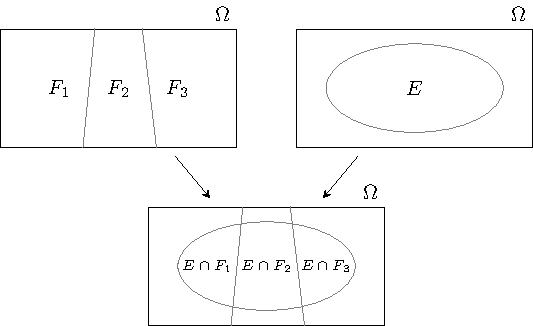
\includegraphics{ds4psy_files/figure-latex/tikz-prob-tot-1} 

}

\caption{Partizione dello spazio campionario $\Omega$.}\label{fig:tikz-prob-tot}
\end{figure}

\begin{exercise}
Si considerino tre urne, ciascuna delle quali contiene 100 palline:

\begin{itemize}
\tightlist
\item
  Urna 1: 75 palline rosse e 25 palline blu,
\item
  Urna 2: 60 palline rosse e 40 palline blu,
\item
  Urna 3: 45 palline rosse e 55 palline blu.
\end{itemize}

\noindent Una pallina viene estratta a caso da un'urna anch'essa scelta a caso. Qual è la probabilità che la pallina estratta sia di colore rosso?

Sia \(R\) l'evento ``la pallina estratta è rossa'' e sia \(U_i\) l'evento che corrisponde alla scelta dell'\(i\)-esima urna. Sappiamo che

\[
{\mbox{P}}(R \mid U_1) = 0.75, \quad {\mbox{P}}(R \mid U_2) = 0.60, \quad {\mbox{P}}(R \mid U_3) = 0.45.
\]

Gli eventi \(U_1\), \(U_2\) e \(U_3\) costituiscono una partizione dello spazio campionario in quanto \(U_1\), \(U_2\) e \(U_3\) sono eventi mutualmente esclusivi ed esaustivi, \({\mbox{P}}(U_1 \cup U_2 \cup U_3) = 1.0\). In base al teorema della probabilità assoluta, la probabilità di estrarre una pallina rossa è dunque

\[
\begin{split}
{\mbox{P}}(R) &= {\mbox{P}}(R \mid U_1){\mbox{P}}(U_1)+{\mbox{P}}(R \mid U_2){\mbox{P}}(U_2)+{\mbox{P}}(R \mid U_3){\mbox{P}}(U_3) \\
&= 0.75 \cdot \frac{1}{3}+0.60 \cdot \frac{1}{3}+0.45 \cdot \frac{1}{3} \\
&=0.60.
\end{split}
\]
\end{exercise}

\hypertarget{il-teorema-di-bayes}{%
\section{Il teorema di Bayes}\label{il-teorema-di-bayes}}

Introduciamo ora il teorema di Bayes considerando un caso specifico per poi esaminarlo nella sua forma più generale. Sia \(\{F_1, F_2\}\) una partizione dello spazio campionario \(\Omega\). Consideriamo un terzo evento \(E \subset \Omega\) con probabilità non nulla di cui si conoscono le probabilità condizionate rispetto ad \(F_1\) e a \(F_2\), ovvero \({\mbox{P}}(E \mid F_1)\) e \(P(E \mid F_2)\). È chiaro per le ipotesi fatte che se si verifica \(E\) deve anche essersi verificato almeno uno degli eventi \(F_1\) e \(F_2\). Supponendo che si sia verificato l'evento \(E\), ci chiediamo: qual è la probabilità che si sia verificato \(F_1\) piuttosto che \(F_2\)?

\begin{figure}[h]

{\centering 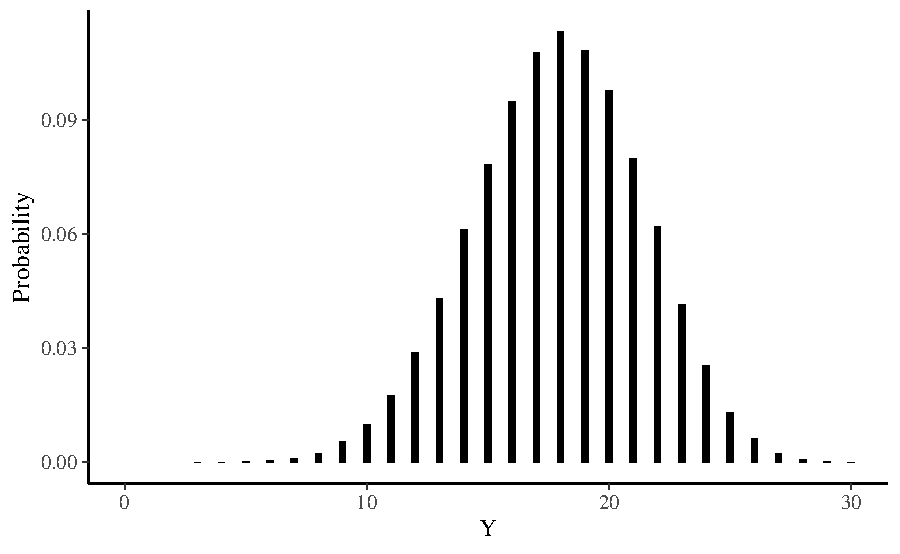
\includegraphics[width=0.45\linewidth]{ds4psy_files/figure-latex/unnamed-chunk-17-1} 

}

\end{figure}

Per rispondere alla domanda precedente scriviamo:

\[
\begin{split}
{\mbox{P}}(F_1 \mid E) &= \frac{{\mbox{P}}(E \cap F_1)}{{\mbox{P}}(E)}\notag\\
              &= \frac{{\mbox{P}}(E \mid F_1){\mbox{P}}(F_1)}{{\mbox{P}}(E)}.
\end{split}
\]

Sapendo che \(E = (E \cap F_1) \cup (E \cap F_2)\) e che \(F_1\) e \(F_2\) sono eventi disgiunti, ovvero \(F_1 \cap F_2 = \emptyset\), ne segue che possiamo calcolare \({\mbox{P}}(E)\) utilizzando il teorema della probabilità assoluta:

\[
\begin{split}
{\mbox{P}}(E) &= {\mbox{P}}(E \cap F_1) + {\mbox{P}}(E \cap F_2)\notag\\
     &= {\mbox{P}}(E \mid F_1)P(F_1) + {\mbox{P}}(E \mid F_2){\mbox{P}}(F_2).
\end{split}
\]

\noindent Sostituendo il risultato precedente nella formula della probabilità condizionata \(P(F_1 \mid E)\) otteniamo:

\begin{equation}
{\mbox{P}}(F_1 \mid E) = \frac{{\mbox{P}}(E \mid F_1){\mbox{P}}(F_1)}{{\mbox{P}}(E \mid F_1){\mbox{P}}(F_1) + {\mbox{P}}(E \mid F_2)P(F_2)}.
\label{eq:bayes1}
\end{equation}

\noindent La \eqref{eq:bayes1} si generalizza facilmente al caso di più di due eventi disgiunti, come indicato di seguito.

\begin{theorem}
Sia \(E\) un evento contenuto in \(F_1 \cup \dots \cup F_k\), dove gli eventi \(F_j, j=1, \dots, k\) sono a due a due incompatibili e necessari. Allora per ognuno dei suddetti eventi \(F_j\) vale la seguente formula:

\begin{equation}
{\mbox{P}}(F_j \mid E) = \frac{{\mbox{P}}(E \mid F_j){\mbox{P}}(F_j)}{\sum_{j=1}^{k}{\mbox{P}}(F_j)P(E \mid F_j)}.
\label{eq:bayes2}
\end{equation}
\end{theorem}

\noindent La \eqref{eq:bayes2} prende il nome di \emph{teorema di Bayes} e mostra che la conoscenza del verificarsi dell'evento \(E\) modifica la probabilità che avevamo attribuito all'evento \(F_j\). Nella \eqref{eq:bayes2} la probabilità condizionata \({\mbox{P}}(F_j \mid E)\) prende il nome di probabilità \emph{a posteriori} dell'evento \(F_j\): il termine ``a posteriori'' sta a significare ``dopo che è noto che si è verificato l'evento \(E\)''.

Nel capitolo \ref{chapter-intro-bayes-inference} estenderemo questa discussione mostrando come la \eqref{eq:bayes2} possa essere formulata nel caso delle variabili casuali continue.

\begin{exercise}
Un lettore attento si sarà reso conto che, in precedenza, abbiamo già applicato il teorema di Bayes, quando abbiamo risolto l'esercizio riportato nella Sezione \ref{sec:bayes-cancer}. Svolgiamo nuovamente lo stesso esercizio applicando ora la \eqref{eq:bayes2} che, per convenienza, riscriviamo come:

\begin{align}
{\mbox{P}}(M \mid +) &= \frac{{\mbox{P}}(+ \mid M) {\mbox{P}}(M)}{{\mbox{P}}(+ \mid M) {\mbox{P}}(M) + {\mbox{P}}(+ \mid M^\complement) {\mbox{P}}(M^\complement)}\notag\\ 
&= \frac{0.9 \cdot 10/1000}{0.9 \cdot 10/1000 + 99 / 990 \cdot 990 / 1000} \notag\\
&= \frac{9}{108}.\notag
\end{align}
\end{exercise}

\hypertarget{commenti-e-considerazioni-finali-2}{%
\section*{Commenti e considerazioni finali}\label{commenti-e-considerazioni-finali-2}}


Il teorema di Bayes rende esplicito il motivo per cui la probabilità non possa essere pensata come uno stato oggettivo, quanto piuttosto come un'inferenza soggettiva e condizionata. Il denominatore del membro di destra della \eqref{eq:bayes2} è un semplice fattore di normalizzazione. Nel numeratore compaiono invece due quantità: \({\mbox{P}}(F_j\)) e \({\mbox{P}}(E \mid F_j)\). La probabilità \({\mbox{P}}(F_j\)) è la probabilità \emph{probabilità a priori} (\emph{prior}) dell'evento \(F_j\) e rappresenta l'informazione che l'agente bayesiano possiede a proposito dell'evento \(F_j\). Diremo che \({\mbox{P}}(F_j)\) codifica il grado di fiducia che l'agente ripone in \(F_j\) prima di avere osservato i dati. Nell'interpretazione bayesiana, \({\mbox{P}}(F_j)\) rappresenta un giudizio personale dell'agente e non esistono criteri esterni che possano determinare se tale giudizio sia coretto o meno. La probabilità condizionata \({\mbox{P}}(E \mid F_j)\) rappresenta invece la verosimiglianza di \(F_j\) e ci dice quant'è plausibile che si verifichi l'evento \(E\) condizionatemente al fatto che si sia verificato \(F_j\). Il teorema di Bayes descrive la regola che l'agente deve seguire per aggiornare il suo grado di fiducia in \(F_j\) alla luce di un ulteriore evento \(E\). La \({\mbox{P}}(F_j \mid E)\) è chiamata probabilità a posteriori dato che rappresenta la nuova probabilità che l'agente assegna ad \(F_j\) affinché rimanga consistente con le nuove informazioni fornitegli da \(E\).

La probabilità a posteriori dipende sia da \(E\), sia dalla conoscenza a priori dell'agente \({\mbox{P}}(F_j)\). In questo senso è chiaro come non abbia senso parlare di una probabilità oggettiva: per il teorema di Bayes la probabilità è definita condizionatamente alla probabilità a priori, la quale a sua volta, per definizione, è un'assegnazione soggettiva. Ne segue pertanto che ogni probabilità debba essere considerata come una rappresentazione del grado di fiducia soggettiva dell'agente. Dato che ogni assegnazione probabilistica rappresenta uno stato di conoscenza e che ciascun particolare stato di conoscenza è arbitrario, un accordo tra agenti diversi non è richiesto. Tuttavia, la teoria delle probabilità ci fornisce uno strumento che, alla luce di nuove informazioni, consente l'aggiornamento dello stato di conoscenza in un modo razionale.

Il teorema di Bayes consente di modificare una credenza a priori in maniera dinamica, via via che nuove evidenze vengono raccolte, in modo tale da formulare una credenza a posteriori la quale non è mai definitiva, ma possa sempre essere aggiornata in base alle nuove evidenze disponibili. Questo processo si chiama \emph{aggiornamento bayesiano}.

\begin{remark}
Qual è la pronuncia di ``Bayesian''? Per saperlo possiamo seguire \href{https://bayes-rules.github.io/posts/fun/}{questo link}.
\end{remark}

\mainmatter

\hypertarget{part-appendici}{%
\part{Appendici}\label{part-appendici}}

\hypertarget{appendix-appendici}{%
\appendix \addcontentsline{toc}{chapter}{\appendixname}}


  \bibliography{refs.bib,book.bib,packages.bib}

\printindex

\end{document}
